\chapter{Efficiency evaluation}
\label{chap:prod:effs}

The efficiency chain defines the fraction of produced prompt signal candidates 
that survive the full reconstruction and selection procedure.
The chain is defined in steps grouped by physical requirements and those 
imposed by software, with each step being relative to the previous one.
In the order of steps by which candidates are lost, this starts with the efficiency of a signal charm hadron to decay within the 
\lhcb\ acceptance having been produced in a \pp\ collision, \effacc.
The efficiency of such a decay to be fully reconstructed is the reconstruction 
efficiency is \effreco, and then the efficiency of the reconstructed decay to 
be triggered through \lzero, \hltone, and \hlttwo is the trigger efficiency 
\efftrig.
Finally, there is the efficiency of triggered candidates to pass through the 
offline selection \effoffline.
The total efficiency, \eff, is the product of these, and is what enters in 
\cref{eqn:prod:introduction:differential_cross_section}.

For most steps in the efficiency chain, the candidates not passing each step 
are lost and cannot be processed further, and so methods are needed to assess the 
efficiency without having access to the original candidates.
There are two methods that shall be used in this \namecref{chap:prod:effs}: 
efficiency estimation from simulated \acf{MC} data, described in 
\cref{chap:prod:data:mc}, where true information is available before and after 
all steps; and methods of calibration, where proxy data selected without the 
use of particular information can be used to assess the effects of using that information in the 
analysis data.
Efficiency evaluation with \ac{MC} can be simple, but differences between the 
data and the \ac{MC} must be accounted for, which may not be obvious.
Calibration techniques use real data, and so can be more robust than \ac{MC}, 
but obtaining clean calibration samples can be challenging.

In \lhcb, it is known that the \ac{PID} selection efficiencies are not 
well-modelled in the \ac{MC}, due to an under-estimation of the detector 
occupancies.
The same is true, albeit to a lesser extent, for the reconstruction 
efficiencies.
Kinematic variables, such as charm hadron and final state momenta, are 
comparatively well-modelled.
This motivates a two-step procedure for evaluating the \emph{selection} 
efficiency, whereby the \ac{PID} efficiency is computed using calibration 
techniques, described in \cref{chap:prod:effs:pid}, and the efficiency of the remaining 
requirements is made using \ac{MC}, detailed in \cref{chap:prod:effs:sel}.
The reconstruction efficiency will be computed using \ac{MC}, but corrected 
with a factor obtained from calibration samples, described in \cref{chap:prod:effs:acc}.
The extent to which these techniques do not accurately model the efficiencies 
will be discussed in the context of systematic uncertainties in 
\cref{chap:prod:syst:mc}.

To summarise: the total efficiency $\eff_{i}(\decay{\PHc}{f})$, for charm candidates in the $i$th \pTy\ bin, is 
the product of the individual efficiencies and correction factors
% TODO should revisit this to include how the sections actually flow; could 
% have the L0 efficiency explicitly, for example
\begin{align}
  \eff_{i}(\decay{\PHc}{f}) = \effacc &\times \effreco \times \efftracking \times \efftrig \nonumber\\
                                      &\times \effoffline \times \effpid.
  \label{eqn:prod:effs:total_eff}
\end{align}
where each efficiency \eff\ is dependent on the charm hadron \PHc\ and the 
final state $f$, and is conditional on the previous step.

In this \namecref{chap:prod:effs} the details of the efficiency computation for each step is 
given, along with example efficiency tables in \pTy\ for the two-body \DzToKpi\ 
and three-body \DpToKpipi\ decays.
The notation for conditional yields will be used throughout, where $N_{A|B}$ 
denotes the prompt signal yields after process $A$ given that process $B$ 
preceded $A$.

\section{Detector acceptance}
\label{chap:prod:effs:acc}

The acceptance efficiency is due to the finite spatial acceptance of the \lhcb\ 
detector.
By instrumenting the forward region, in the pseudorapidity range $2 < \Eta < 
5$, any particles flying outside this region are not detected.
As there is no way to access these particles in data, it is necessary to use 
simulated data.
The acceptance is modelled by a set of cuts requiring that all stable charged 
particles in the final state are within $10 < \theta < 
\SI{400}{\milli\radian}$, where $\theta$ is the polar angle of the particle 
momentum vector, and that all the particles in the final state point in the 
positive $z$ direction, as defined in \cref{chap:prod:data:mc}.
These requirements are applied at the \emph{generator} level, before the 
detector simulation, on the true kinematics of the particles.

By counting the number of charm hadrons passing and failing the cut, the 
acceptance efficiency is defined as
\begin{equation}
  \effacc = \frac{%
    N_{\text{Accepted}|\text{Generated}}
  }
  {%
    N_{\text{\text{Generated}}}
  }.
  \label{eqn:prod:effs:acc}
\end{equation}
The input dataset to this computation is the generator-level set described in 
\cref{chap:prod:data:mc}.
% TODO should mention that we're using AC intervals, stating why and what they
% are
The acceptance efficiencies for \DzToKpi\ and \DpToKpipi, in \pTy\ bins, are 
given in \cref{tab:prod:effs:acc:dztokpi,tab:prod:effs:acc:dptokpipi}.

\section{Reconstruction}
\label{chap:prod:effs:reco}

The reconstruction efficiency \effreco\ parameterises the fraction of charm meson decays passing the acceptance requirements that are also fully reconstructed as tracks, for the final state particles, and vertices, for the charm mesons.
This folds in several effects: whether the final state particles have a large enough momentum not to be bent out of the detector acceptance by the magnetic field; whether the final state particles leave enough hits in the tracking system to be \emph{reconstructible} (that is, above the minimum threshold at which the tracking system \emph{could} reconstruct a track); whether, given that enough hits were deposited by a final state particle, a track was actually \emph{reconstructed}; and whether a vertex can be formed, given that all final state particles have associated tracks.
The reconstruction efficiency can be defined as the ratio of fully reconstructed decays to those passing the acceptance requirements
\begin{equation}
  \effreco = \frac{%
    N_{\text{Reconstructed}|\text{Accepted}}
  }
  {%
    N_{\text{\text{Accepted}}}
  }.
  \label{eqn:prod:effs:reco}
\end{equation}
The reconstruction efficiencies for \DzToKpi\ and \DpToKpipi, in \pTy\ bins, are 
given in \cref{tab:prod:effs:reco:dztokpi,tab:prod:effs:reco:dptokpipi}.

\subsection{Truth matching inefficiency}
\label{chap:prod:effs:truth}

The evaluation of \cref{eqn:prod:effs:reco} requires that the reconstructed objects, tracks and vertices, be correctly associated back to the `truth-level' information, that is the \ac{MC} objects which were generated and then propagated through the detector simulation.
The truth-matching procedure is described in \cref{chap:prod:data:mc}.
The background category information is used to filter the \ac{MC} such that the 
number of remaining candidates are counted to obtain the input to some 
efficiency computation, such as \cref{eqn:prod:effs:reco}.
However, the requirement that a track is matched to \SI{70}{\percent} of the hits created by an \ac{MC} particle is not \SI{100}{\percent} efficient at accepting signal.
This results in an underestimation of the number of signal particles, and hence an overestimation of the cross-section.
The magnitude of the size of the inefficiency can be determined by counting the 
number of signal yields that fail the truth matching requirement.
\cref{fig:prod:effs:truth:categories} shows the \PDzero and \PDplus mass 
distributions for the various background categories.
The only signal-like background category is the `ghost' category,
where the vertex was made from at least one track that was determined to be a ghost track.

Given that the number of correctly matched signal decays is $N$, and the number 
of incorrectly labelled signal decays is $U$, the selection efficiency defined 
in \cref{eqn:prod:effs:reco} is incorrect by a factor
\begin{equation}
  \efftruth = \frac{U+N}{N}.
  \label{eqn:prod:effs:truth}
\end{equation}
The number of decays passing the signal requirement is used for $N$, and $U$ 
can be measured with a maximum likelihood fit to mass distribution of the 
decays not passing that requirement.
As shown in \cref{fig:prod:effs:truth:categories}, the fraction of incorrectly 
identified signal decays is small, and so a single fit is performed with the 
data integrated across all \pTy\ bins.
The details of the fit are identical to those for the mass fits used in the 
prompt charm yield extraction with real data, described in 
\cref{chap:prod:fitting}.
The result of the fits to the \DzToKpi\ and the \DpToKpipi\ simulated datasets 
are shown in \cref{fig:prod:effs:truth:fit}.
Table~\ref{tab:prod:effs:truth_matching} lists the obtained efficiencies.

\begin{figure}
  \begin{subfigure}[b]{0.5\textwidth}
    \centering
    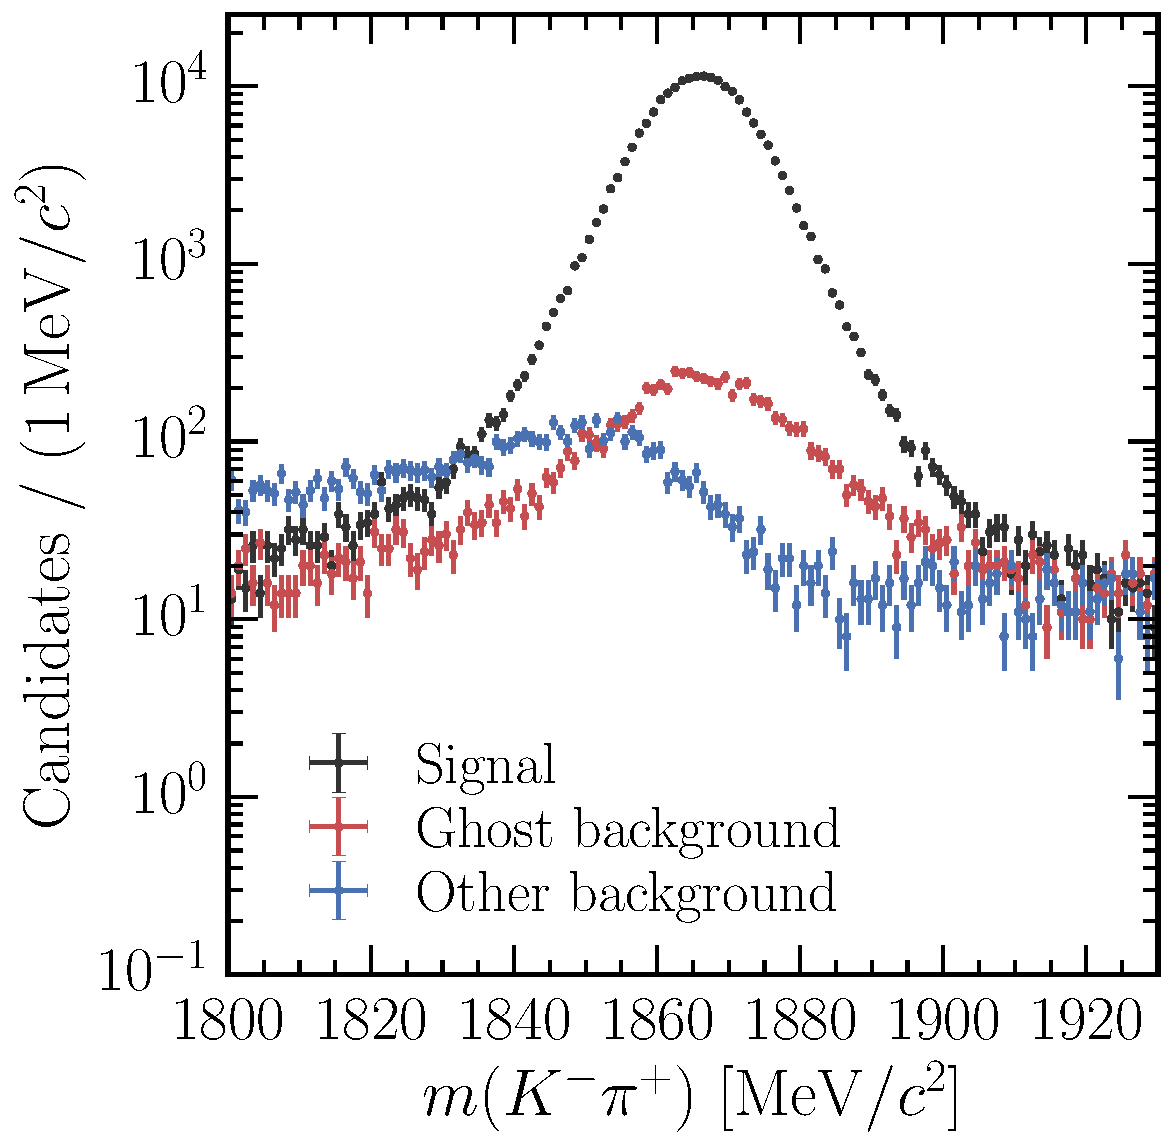
\includegraphics[width=\textwidth]{production/efficiencies/D0ToKpi_BKGCAT}
    \caption{\PDzero}
    \label{fig:prod:effs:truth:categories:D0ToKpi}
  \end{subfigure}
  \begin{subfigure}[b]{0.5\textwidth}
    \centering
    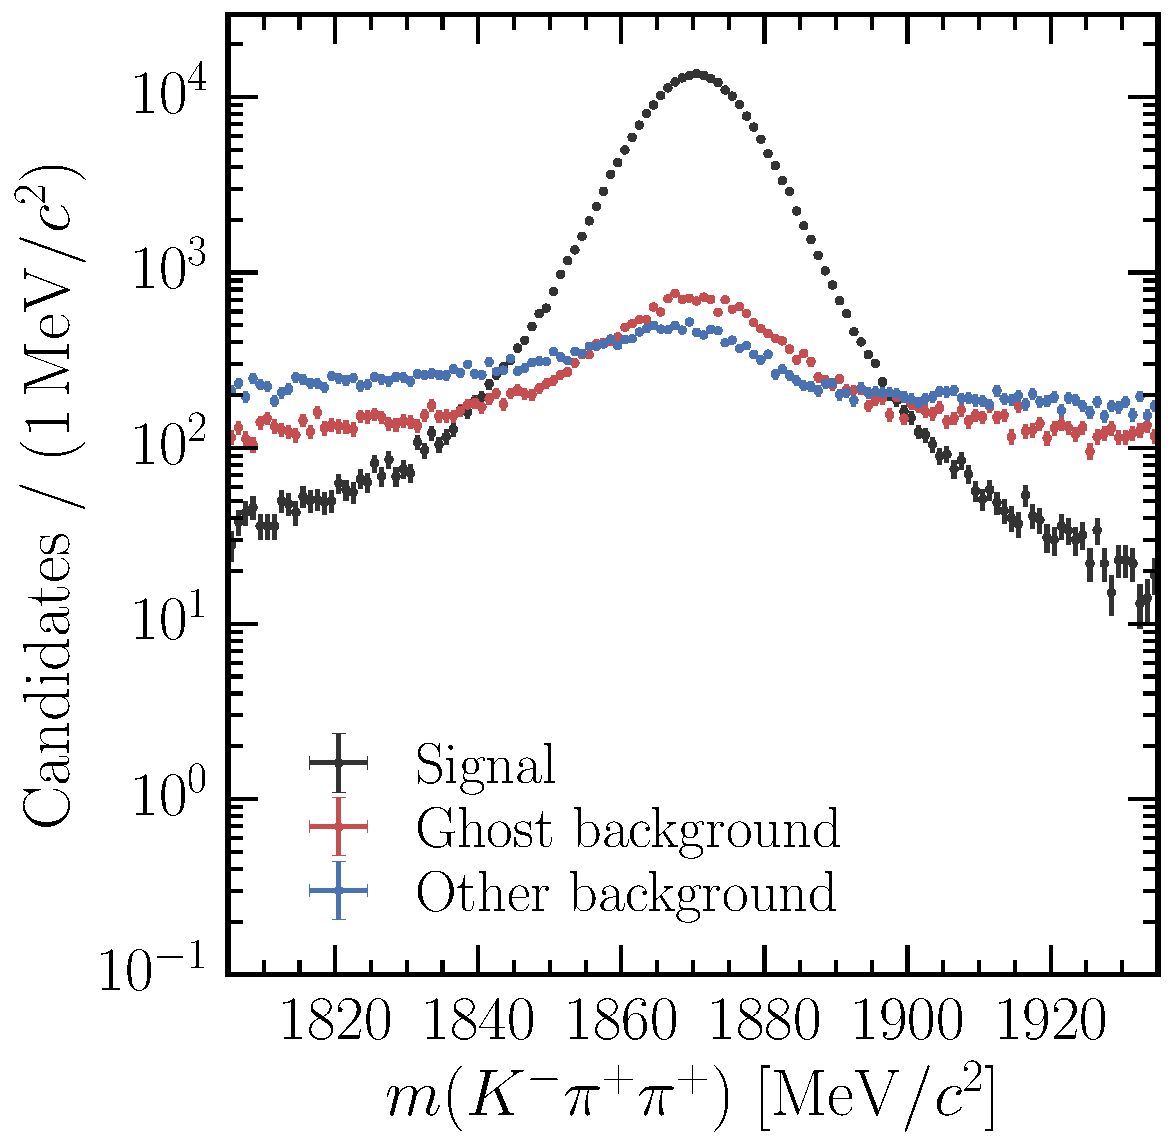
\includegraphics[width=\textwidth]{production/efficiencies/DpToKpipi_BKGCAT}
    \caption{\PDplus}
    \label{fig:prod:effs:truth:categories:DpToKpipi}
  \end{subfigure}
  \caption{%
    Mass distributions of \ac{MC} 
    \PDzero~(\subref*{fig:prod:effs:truth:categories:D0ToKpi}) and 
    \PDplus~(\subref*{fig:prod:effs:truth:categories:DpToKpipi}) candidates for 
    various background categories, as indicated in the legends.
    The most prominent features are the signal-like peak in the `ghost' 
    distribution, indicative of a truth-matching inefficiency, and the long 
    tail extending below the mass peak in the `other' distribution, which 
    mostly consists of partially reconstructed physics backgrounds such as 
    \decay{\PDzero}{\PKminus\Ppiplus\Ppizero} and 
    \decay{\PDplus}{\PKminus\Ppiplus\Ppiplus\Ppizero}.
  }
  \label{fig:prod:effs:truth:categories}
\end{figure}

\begin{figure}
  \begin{subfigure}[b]{0.5\textwidth}
    \centering
    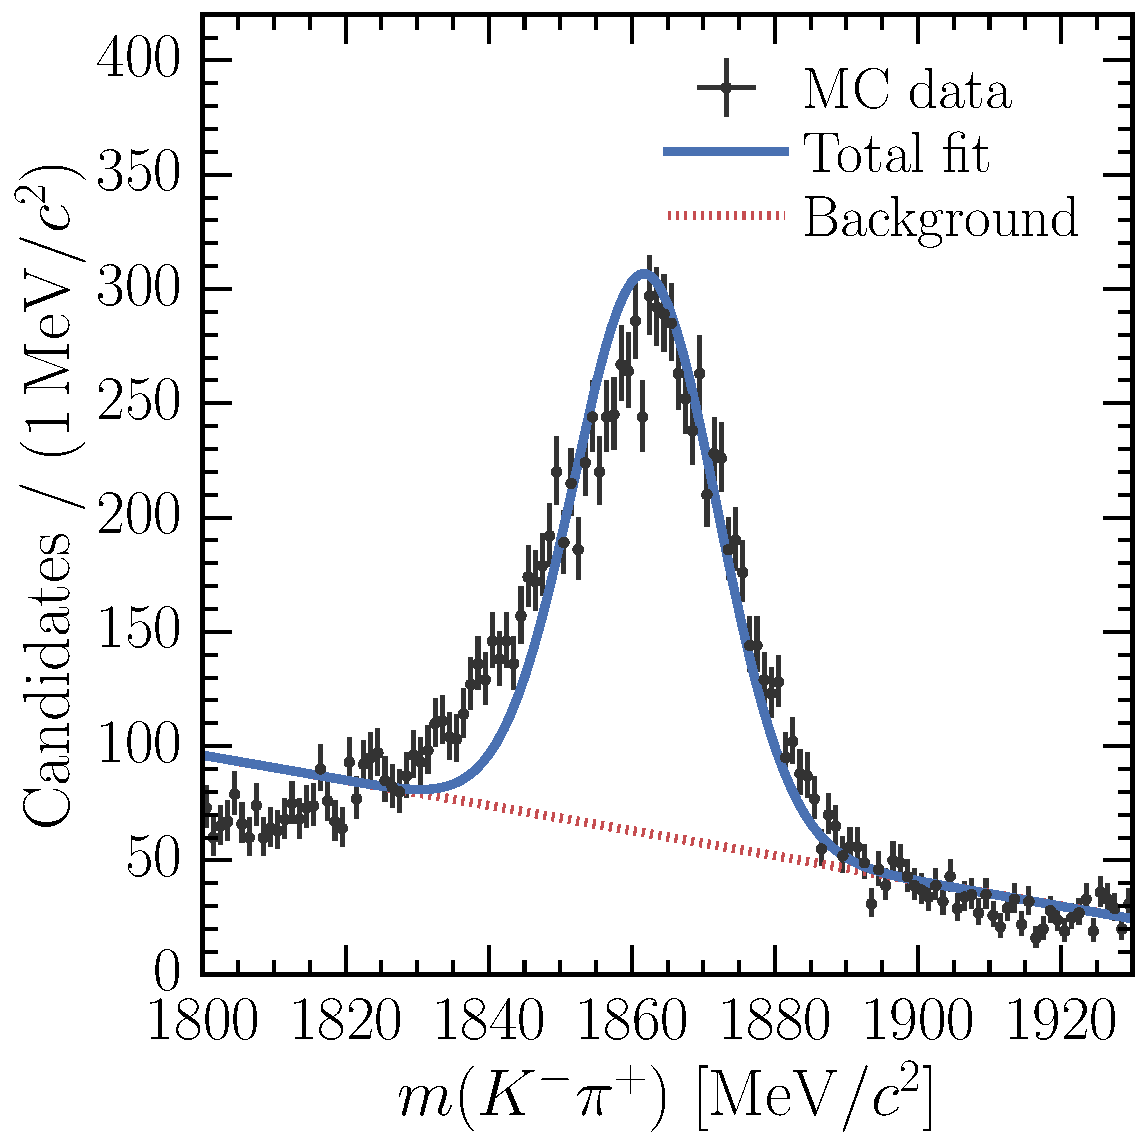
\includegraphics[width=\textwidth]{production/efficiencies/D0ToKpi_BKGCAT_fit}
    \caption{\DzToKpi}
    \label{fig:prod:effs:truth:fit:D0ToKpi}
  \end{subfigure}
  \begin{subfigure}[b]{0.5\textwidth}
    \centering
    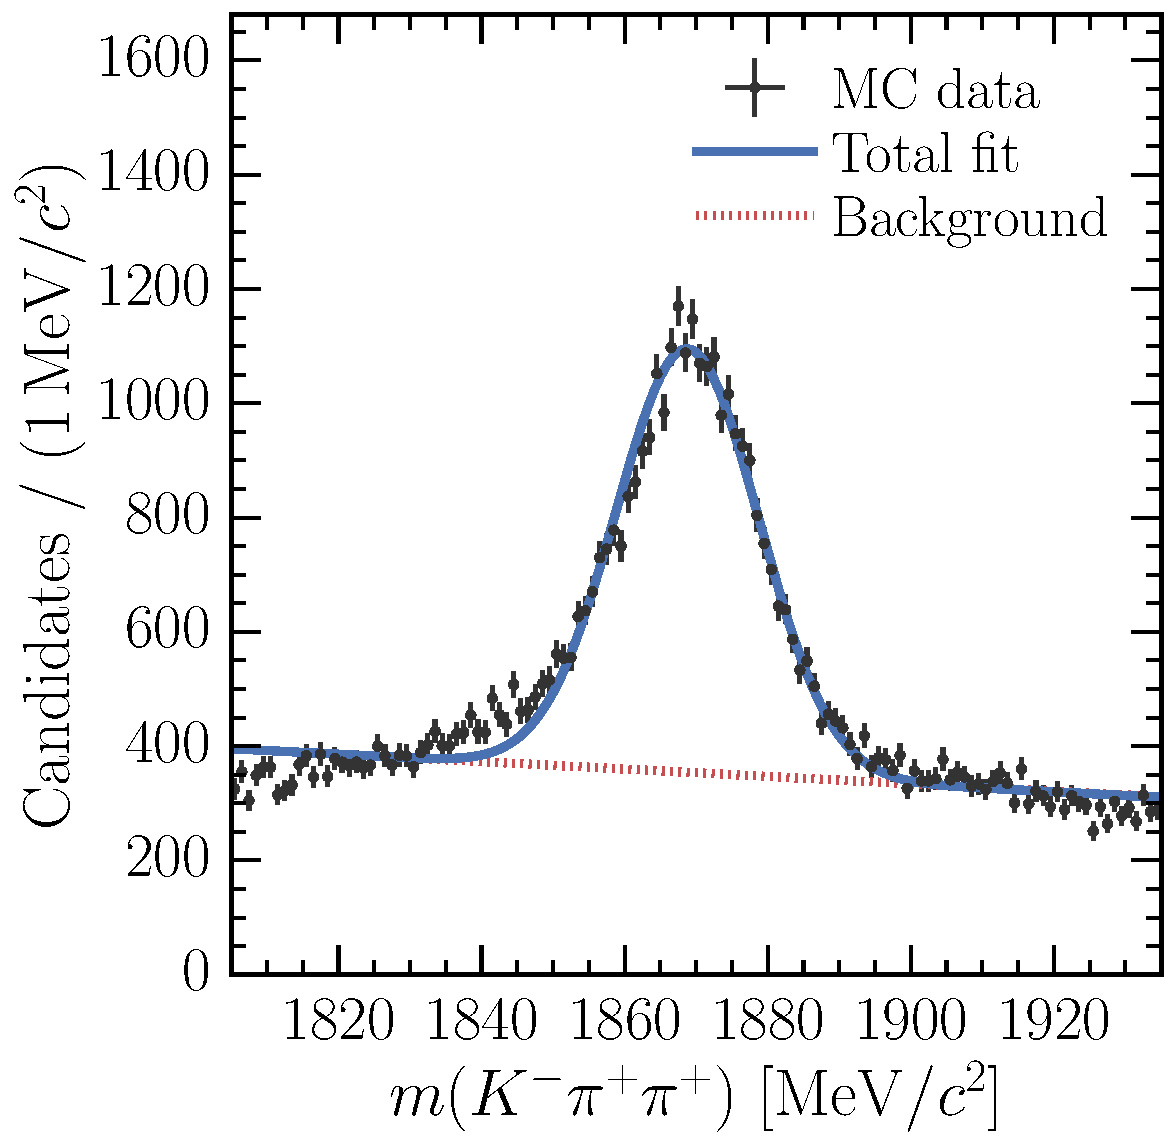
\includegraphics[width=\textwidth]{production/efficiencies/DpToKpipi_BKGCAT_fit}
    \caption{\DpToKpipi}
    \label{fig:prod:effs:truth:fit:DpToKpipi}
  \end{subfigure}
  \caption{%
    Mass distributions of \ac{MC} 
    \PDzero~(\subref*{fig:prod:effs:truth:fit:D0ToKpi}) and 
    \PDplus~(\subref*{fig:prod:effs:truth:fit:DpToKpipi}) candidates not 
    passing the `signal' truth-matching requirement, that is the sum of the 
    ``Ghost'' and ``Other'' categories shown in 
    \cref{fig:prod:effs:truth:categories}.
    Overlaid on each distribution is the result of a maximum likelihood fit, 
    with the total \acl{PDF} shown as a blue curve, and the background 
    \acl{PDF} as a red curve.
  }
  \label{fig:prod:effs:truth:fit}
\end{figure}

\subsection{Tracking efficiency correction}
\label{chap:prod:effs:tracking}

The track reconstruction efficiency, or \emph{tracking efficiency}, 
measurements the efficiency for a charged particle to be reconstructed as a 
track, and is part of the definition of the reconstruction efficiency in 
\cref{eqn:prod:effs:reco}.
The \ac{MC} may not accurately model the tracking efficiency, and so a 
data-driven technique is used to create correction factors based on the 
observed differences between the data and the \ac{MC}.

Only \emph{long} tracks are used in this analysis, which requires the particles 
to creates hits in the \velo\ and in the T stations.
Hits in the \ttracker\ are not required to form long tracks, though the 
information can be used to improve the momentum resolution.
To probe the efficiency of long track creation, \JpsiTomumu\ decays are 
reconstructed using a `tag-and-probe' technique, where one particle is fully 
reconstructed as a long track, as usual, and the other track is created using 
track segments made only using information from the muon stations.
The momentum of the latter track, the `probe', can be inferred by treating the 
magnetic field as an optical system that imparts a momentum `kick' in the $x$ 
direction.
By assuming the muon track segment was made by a particle originating from the 
\ac{PV}, the probe segment can be extrapolated back from the muon stations to 
the $yz$ plane where the kick is modelled, and then the difference in slopes 
between the \ac{PV}-plane line and the probe track gives the probe momentum.
The invariant mass of the dimuon system can then be computed, the distribution 
of which for many tag-and-probe candidates can be used to distinguish between 
backgrounds and true \PJpsi decays.
The mass resolution of \JpsiTomumu\ decays reconstructed using long+muon tracks 
is about \SI{200}{\MeVcc}, to be compared with a resolution of about 
\SI{16}{\MeVcc} using long+long tracks.
To improve the mass resolution, the muon tracks are combined with hits in the 
\ttracker, improving the resolution to around 
\SI{57}{\MeVcc}~\cite{Aaij:2014pwa,DeCian:2013zua}.

The tracking efficiency is evaluated as the ratio of \PJpsi mesons 
reconstructed using the long+muon+\ttracker\ method, with those that can also 
be reconstructed using the long+long method
\begin{equation}
  \eff_{\text{Tracking}} = 
  \frac{%
    N_{\text{long+long|long+muon+TT}}
  }{%
    N_{\text{long+muon+TT}}
  }.
  \label{eqn:prod:effs:tracking_eff}
\end{equation}
A long track an event is considered as `matched' to the probe track if there is 
a \SI{70}{\percent} overlap of their hits in the muon stations.
This tag-and-probe method is performed using real data and \ac{MC}, and a ratio 
is formed
\begin{equation}
  \efftracking = \frac{%
    \eff_{\text{Tracking}}^{\text{Data}}
  }{%
    \eff_{\text{Tracking}}^{\text{MC}}
  }.
  \label{eqn:prod:effs:tracking_ratio}
\end{equation}
This ratio is evaluated in bins of probe track momentum \ptot\ and 
pseudorapidity \Eta, as the tracking efficiency is found to vary strongly as a 
function of these variables, and is shown in 
\cref{fig:prod:effs:tracking_table}.
As it is also found to vary as a function of the total number of reconstructed 
long tracks in the event, the input tracks in the \ac{MC} are weighted such 
that event multiplicity distribution matches that in the data.

The correction factor in \cref{eqn:prod:effs:tracking_ratio} can be applied to 
the tracking efficiency found using any decay, as it is only a function of 
\ptot\ and \Eta.
It is then applied to the reconstruction efficiency in 
\cref{eqn:prod:effs:reco}, where for a single decay the total correction factor 
is the product of the correction factors for all the tracks comprising the 
final states.
Tracking efficiency correction factors for \DzToKpi\ and \DpToKpipi\ are given 
in \cref{tab:prod:effs:tracking:dztokpi,tab:prod:effs:tracking:dptokpipi}.

The correction factors given do not account for the differences between muon 
and hadron interactions with the detector.
These differences will result in different tracking efficiencies, which may not 
be the same between data and \ac{MC}.
The effect of these differences will be discussed in the context of systematic 
uncertainties in \cref{chap:prod:syst:tracking}.

\begin{figure}
  \centering
  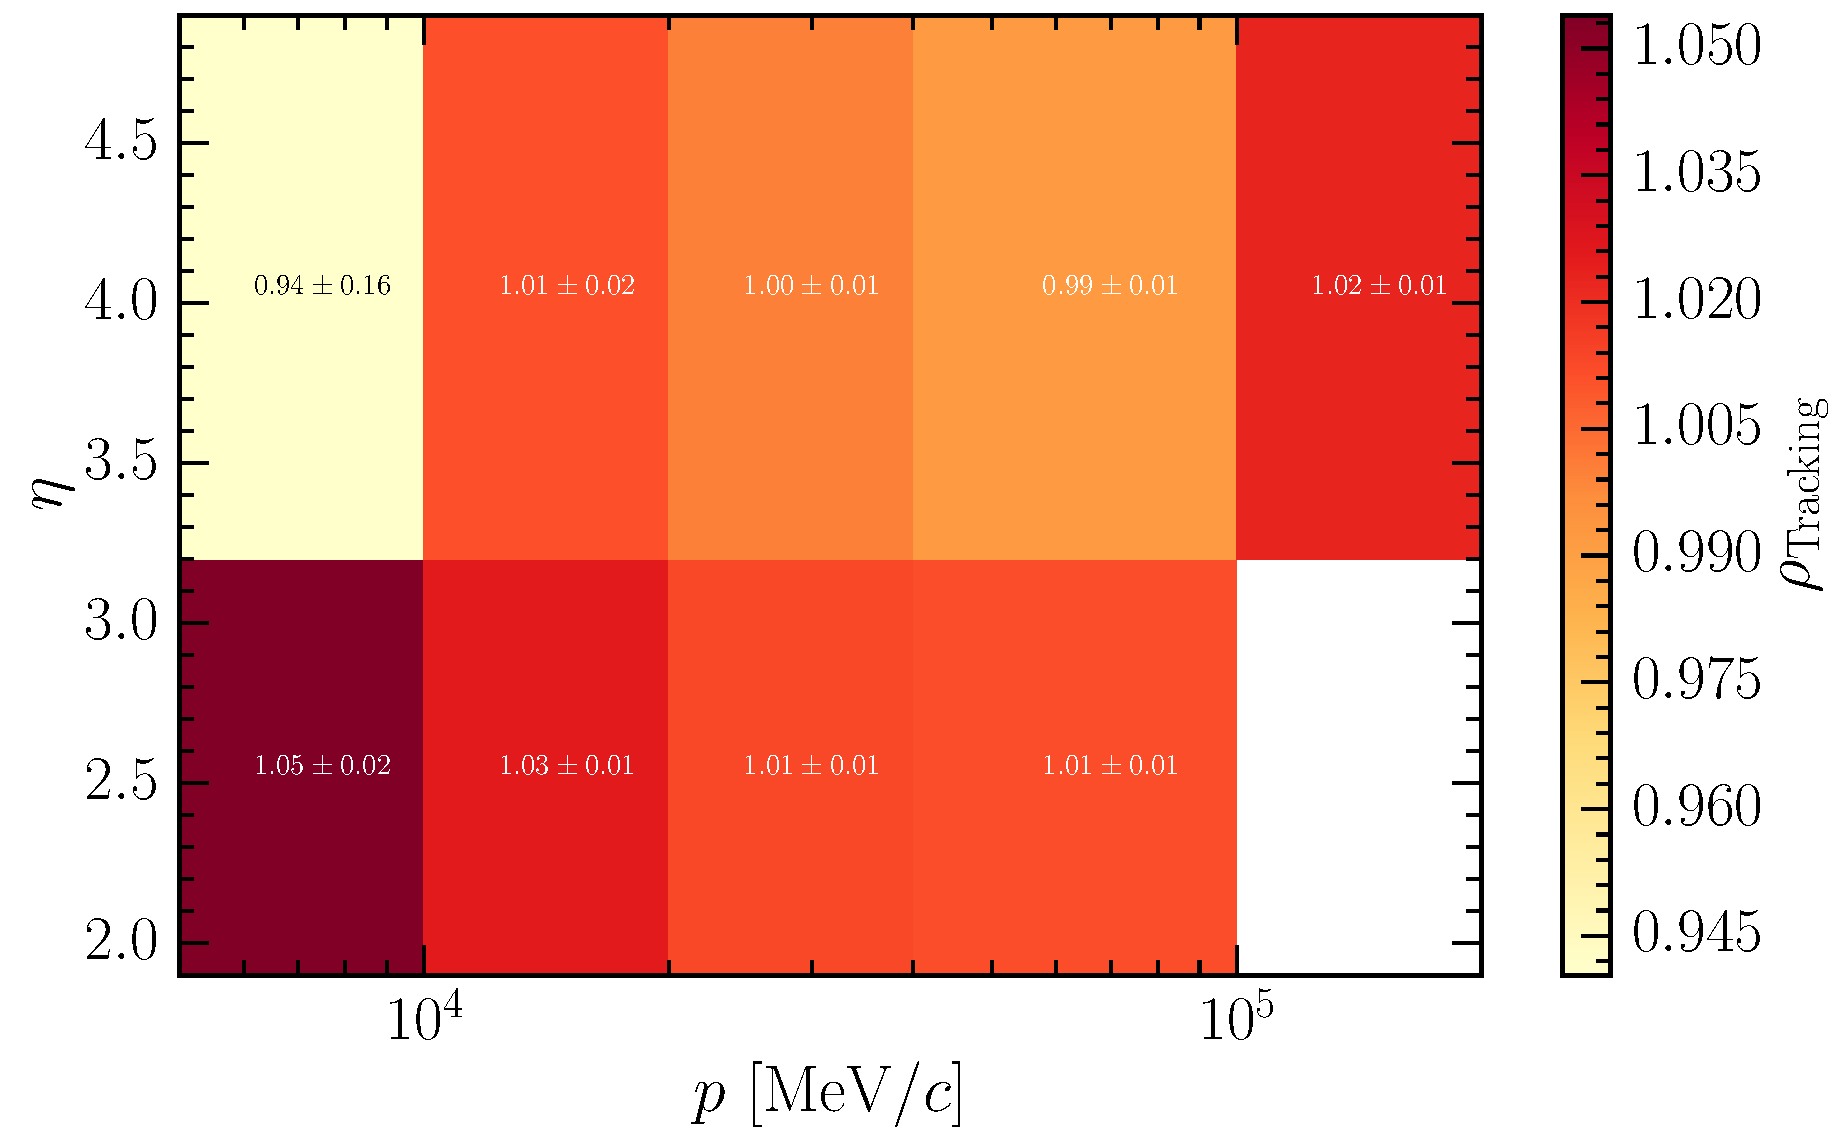
\includegraphics[width=\textwidth]{production/efficiencies/tracking_correction_table}
  \caption{%
    Tracking efficiency correction factors \efftracking\ in bins of track 
    momentum and pseudorapidity.
    The value is labelled in each bin, along with the statistical uncertainty 
    on those values due to the finite size of the calibration datasets.
    Bins in which a measurement could not be made are empty.
  }
  \label{fig:prod:effs:tracking_table}
\end{figure}

Combining the truth-matching efficiency and tracking efficiency correction 
factors, the reconstruction efficiency is redefined from 
\cref{eqn:prod:effs:reco} to be
\begin{equation}
  \effreco = \efftruth\times\efftracking\times\frac{%
    N_{\text{Reconstructed}|\text{Accepted}}
  }
  {%
    N_{\text{\text{Accepted}}}
  }.
  \label{eqn:prod:effs:reco_corrected}
\end{equation}

\section{Selection}
\label{chap:prod:effs:sel}

At this stage, the efficiency chain includes the effects of the detector 
acceptance, of the reconstruction, of the truth-matching used to evaluate the 
reconstruction efficiency, and of the data-\ac{MC} differences in the tracking 
efficiency.
What it left is the selection efficiencies due to the online and offline 
selections, as described in \cref{chap:prod:sel}.
For simplicity, the `online' and `offline' selection are treated as a single 
requirement, with the caveat any \ac{PID} requirements are not included.
The \ac{PID} efficiency can be computed using data-driven methods, and will be 
described in \cref{chap:prod:effs:pid}.

The \lzero\ trigger selects bunch-bunch crossings randomly at a predetermined 
rate, and so the \lzero\ efficiency is just the ratio of accepted crossings to 
the total number, or equivalently
\begin{equation}
  \eff_{\lzero} = \frac{%
    R_{\nobias}
  }{%
    \ncollbunches\revfreq
  },
  \label{eqn:prod:effs:sel:l0}
\end{equation}
where $R_{\nobias}$ is the rate at which the \lzero\ trigger was programmed to 
accept crossings; \ncollbunches\ is the number of bunches in the \ac{LHC} which 
collided at the \lhcb\ \acl{LHCIP}; and \revfreq\ is the bunch revolution 
frequency of \SI{11.246}{\kilo\hertz}.
Both $R_{\nobias}$ and \ncollbunches\ can vary as a function of the \ac{LHC} 
fill, and hence so can $\eff_{\nobias}$.
The corresponding values are tabulated in 
\cref{tab:prod:sel:online:l0_nobias_rateeff}.

The remaining \hltone, \hlttwo, and offline selection efficiency is computed as 
the ratio of the number of truth-matched decays passing the full selection (but 
without \ac{PID} requirements) to the number of truth-matched, reconstructed 
decays, giving
\begin{equation}
  \effselection = \frac{%
    N_{\text{Selected}|\text{Reconstructed}}
  }{%
    N_{\text{Reconstructed}}
  }.
  \label{eqn:prod:effs:sel}
\end{equation}
Selection efficiencies for \DzToKpi\ and \DpToKpipi\ are given in 
\cref{tab:prod:effs:sel:dztokpi,tab:prod:effs:sel:dptokpipi}.

\section{Particle identification}
\label{chap:prod:effs:pid}

The efficiency of a requirement on one of the variables that is discriminatory 
between charged particle species is the \ac{PID} efficiency \effpid.
The variables are those in the \acf{DLL} family, of which this analysis uses 
the \dllkpi\ variable to define all kaon and pion tracks, with the exception of 
the soft pion in the \DstToDzpi decay.
This \namecref{chap:prod:effs:pid} shall describe how the \effpid\ is computed.

It is assumed that the efficiency of a \ac{PID} cut for a given particle type 
can be parameterised as a function of three variables: the track momentum 
\ptot, the track pseudorapidity \Eta, and a measure of the detector occupancy.
These particular variables are chosen as the performance of the \rich\ 
detectors is known to depend them~\cite{Adinolfi:2012qfa}.
As a measure of the detector occupancy, the number \nspd\ of hits in the \spd\ 
detector is used.
If a model can be constructed of the efficiency for a particular \ac{PID} 
requirement as a function of \ptot, \Eta, and \nspd, this model can then be 
used to determine the \ac{PID} efficiency of that requirement for any sample.

A clean sample of \DzToKpi\ decays can be obtained without the use of \ac{PID} 
information.
This sample will be referred to here as the \emph{calibration} sample, and a 
has a small overlap, around \SI{20}{\percent}, with the sample used for the 
cross-section measurement, due to the different selection strategy that is 
required when \ac{PID} information is ignored.
To compute the efficiency of a given \ac{PID} requirement on either a kaon or a 
pion track, kaons or pions from the calibration sample are partitioned in 
\ptot, \Eta, and \nspd as a three-dimensional histogram.
The number of signal tracks $C_{i}$ in the $i$th bin is computed, and then the 
number of signal decays after the \ac{PID} requirement $C_{i}'$ is computed, 
such that the efficiency in the $i$th bin is
\begin{equation}
  \eff_{i} = \frac{C_{i}'}{C_{i}}.
\end{equation}
It is assumed that the $(\ptot,\,\Eta,\,\nspd)$ partitions are sufficiently 
small that the \ac{PID} efficiency within a bin is single-valued.

One method to obtain the track counts $C_{i}$ and $C_{i}'$ is to perform a 
likelihood fits to the $\PKminus\Ppiplus$ invariant mass distribution, before 
and after the \ac{PID} requirement, where the signal \PDzero decays can be 
modelled as a peaking structure and the combinatorial background can be 
modelled as linear or exponential.
This can take a substantial amount of time, however, as many fits must be 
performed and checked.
Instead, a single fit is run on the entire calibration sample, and weights are 
computed that can be used to statistically remove the background contribution 
in variable distributions that are uncorrelated with the invariant 
mass.\footnotemark
As \ptot, \Eta, and \nspd\ are found to be uncorrelated with 
$m(\PKminus\Ppiplus)$, these weights can be used to compute $C_{i}$ by summing 
the weights of the tracks that fall in the $i$th bin.
They can also be used to compute $C_{i}'$ in the same way, as the \dll\ 
variables are also found to be uncorrelated with $m(\PKminus\Ppiplus)$, and a 
cut on a variable is the same as partitioning data into bins.
Once the efficiency in each $(\ptot,\,\Eta,\,\nspd)$ bin is computed, the 
\ac{PID}\ efficiency for the same cut can be computed for a track from 
\emph{any} source by looking up which bin it falls into, and assigning the 
corresponding efficiency to it.

\footnotetext{%
  These weights are called \emph{sWeights}~\cite{Pivk:2004ty}.
  % TODO should reference a specific chapter where sWeights are described
  A more complete description of their computation, properties, and use cases 
  will be given in \cref{chap:cpv}.
}

For the calibration sample, the average efficiency across the parameterisation 
space can be expressed as
\begin{equation}
  \effpid = \frac{%
    \displaystyle\sum_{i \in \textnormal{bins}} C_{i}\eff_{i}
    }{%
    \displaystyle\sum_{i \in \textnormal{bins}} C_{i}
    }
\end{equation}
For some other sample of tracks, referred to here as the \emph{reference} 
sample,\footnotemark\ each bin can be assigned a weight $\omega_{i}$ based on 
the fraction of the total sample size in the $i$th bin relative to that for the 
calibration sample
\begin{equation}
  \omega_{i} = \frac{%
    R_{i}
  }{%
    C_{i}
  }\frac{%
    C
  }{%
    R
  },
  \label{eqn:prod:effs:pid:ref_weight}
\end{equation}
where $C_{i}$ ($R_{i}$) is the number of signal calibration (reference) tracks 
in the $i$th bins, as before, and $C$ ($R$) is the total number of signal 
calibration (reference) tracks in the sample.
The average \ac{PID} efficiency for the weighted reference sample is then
\begin{equation}
  \effpid = \frac{%
    \displaystyle\sum_{i \in \textnormal{bins}} \omega_{i}C_{i}\eff_{i}
  }{%
    \displaystyle\sum_{i \in \textnormal{bins}} \omega_{i}C_{i}
  }.
  \label{eqn:prod:effs:pid:single_track_ref_eff}
\end{equation}

\footnotetext{%
  It is the ``reference'' sample because it does not have to be equal to the 
  sample of tracks in data one wishes to know the efficiencies for.
  It can be a sample of simulated data that describes the kinematics of the 
  decay well, or even a different decay mode with similar properties (often 
  called a control channel or a reference channel).
}

For this cross-section analysis, all the final states have multiple charged 
tracks, of different species, upon which \ac{PID} requirements are made.
\Cref{eqn:prod:effs:pid:single_track_ref_eff} gives the average \ac{PID} 
efficiency for a final state where a \ac{PID} requirement is made only on one 
track, and so the formalism must be extended to the multi-track case.
The average efficiency is first modified by substituting 
\cref{eqn:prod:effs:pid:ref_weight} into 
\cref{eqn:prod:effs:pid:single_track_ref_eff}
\begin{equation}
  \effpid = \frac{%
    \displaystyle\sum_{i \in \textnormal{bins}} R_{i}\eff_{i}
  }{%
    \displaystyle\sum_{i \in \textnormal{bins}} R_{i}
  }
  = \frac{1}{R}\sum_{i \in \textnormal{bins}} R_{i}\eff_{i},
\end{equation}
and then expanded in terms of $a_{ij}$, the \emph{weight} of the $j$th 
reference \emph{event} (one set of final state tracks) in the $i$th 
$(\ptot,\,\Eta,\,\nspd)$ bin
\begin{equation}
  \effpid = \frac{1}{R}
            \sum_{i \in \textnormal{bins}}\sum_{j} a_{ij}\eff_{i}.
  \label{eqn:prod:effs:pid:expanded_ref_eff}
\end{equation}
The weight term accounts for the possibility of an impure reference sample, 
where, for example, it can be the same type of weight as used for the creating 
the efficiency histogram from the calibration sample.
The \ac{PID} efficiency calculation can then be thought of as either of two 
equivalent methods: weighting the calibration to look like the reference 
sample, as in \cref{eqn:prod:effs:pid:single_track_ref_eff}, or assigning 
per-event efficiencies to the reference sample based on 
$(\ptot,\,\Eta,\,\nspd)$ bins they fall into, as in 
\cref{eqn:prod:effs:pid:expanded_ref_eff}.
\Cref{eqn:prod:effs:pid:expanded_ref_eff} can be generalised to multi-track 
efficiencies by having the $i$th bin index run over the bins for all particle 
types in the event.
The per-event efficiency $\eff_{e}$ for a multi-track event is the product of 
the individual track efficiencies $\eff_{t}$
\begin{equation}
  \eff_{e} = \prod_{t \in \textnormal{tracks}} \eff_{t}.
\end{equation}
% TODO finish this section

\section{Signal window}
\label{chap:prod:effs:signal_window}

As described in Section~\ref{chap:prod:fitting}, the number of prompt signal 
candidates is measured by fitting the \lnipchisq\ distribution of candidates in 
a signal window defined in the mass distribution.
This mass window requirement removes some signal candidates.
The efficiency of the requirement is evaluated by computing the fractional 
integral of the signal component of the model $f_{\text{Sig.}}(m)$ fitted to 
the mass distribution
\begin{equation}
  \effsigwin = \frac{%
    \int_{M - \delta_{M}}^{M +\delta_{M}} f_{\text{Sig.}}(m) \dif{m}
  }{%
    \int_{-\infty}^{\infty} f_{\text{Sig.}}(m) \dif{m}
  }
  = \int_{M - \delta_{M}}^{M +\delta_{M}} f_{\text{Sig.}}(m) \dif{m},
    \label{eqn:prod:effs:signal_window}
\end{equation}
where $M$ is the nominal charm meson mass, on which the signal window is 
centred, and $\delta_{M}$ is half the width of the signal window.
In the case of the \PDstarp measurement, there is an additional requirement 
that the candidates used in the \lnipchisq\ fit fall in a signal window defined 
in the \deltam\ distribution.
The efficiency of the \deltam\ signal window requirement is computed in the 
same way as for the mass signal window requirement, except the signal component 
of the model fitted to the \deltam\ distribution $g_{\text{Sig}}(\deltam)$ is 
used.
The total signal window for the \PDstarp\ measurement is then
\begin{equation}
  \effsigwin^{\PDstarp} =
    \int_{\deltam_{0} - \delta_{\deltam}}^{\deltam_{0} +\delta_{\deltam}} g_{\text{Sig.}}(\deltam) \dif{\deltam}
    \int_{M - \delta_{M}}^{M +\delta_{M}} f_{\text{Sig.}}(m) \dif{m},
    \label{eqn:prod:effs:signal_window:dst}
\end{equation}
where $\deltam_{0}$ is the nominal \PDstarp-\PDzero mass difference, and $\delta_{\deltam}$ is half the width of the \deltam\ window.

The integral of a probability density function, as in \cref{eqn:prod:effs:signal_window,eqn:prod:effs:signal_window:dst}, is a number.
To assign an uncertainty to this number, the fractional integral is recomputed 
in a series of 500 pseudo-experiments.
Within each one, each shape parameter is assigned a value sampled from a 
normal distribution with a mean as the `nominal' value of that parameter, the 
value found by the fit, and with a width equal to the uncertainty on that nominal 
value. Correlations between the different shape parameters are taken into account.
The variance on the deviation of the integrals, with respect to the integral 
computed using the nominal shape parameter values, is taken as the square of 
the uncertainty on the nominal integral value.

As the shape of some mass signal models are \pTy\ bin dependent, as described 
in Section~\ref{chap:prod:fitting:details}, the signal window efficiency is computed 
separately in each \pTy\ bin.
\Cref{tab:prod:effs:sigwin:dztokpi,tab:prod:effs:sigwin:dptokpipi}
give the per-bin signal window efficiencies for each mode.

\section{Combination of efficiencies}
\label{chap:prod:effs:tot}

% TODO describe how we actually compute the reco+sel eff as one step, and how
% uncertainties are treated (i.e. not using the standard binomial approach)
% TODO normalise tables. D+ tables use [0, 1000[, D0 use [0, 1000]

% These tables are big and ugly, so stick them all at the end of the Chapter
\begin{table}
  \caption{%
    Acceptance efficiencies \effacc\ for \DzToKpi\ measured in \PDzero \pTy\ 
    bins.
  }
  \label{tab:prod:effs:acc:dztokpi}
  \centering
  \renewcommand{\arraystretch}{1.3}
\begin{tabular}{lr@{\hskip+0.2em}c@{\hskip+0.2em}r@{\hskip+0.2em}c@{\hskip+0.2em}rr@{\hskip+0.2em}c@{\hskip+0.2em}r@{\hskip+0.2em}c@{\hskip+0.2em}rr@{\hskip+0.2em}c@{\hskip+0.2em}r@{\hskip+0.2em}c@{\hskip+0.2em}rr@{\hskip+0.2em}c@{\hskip+0.2em}r@{\hskip+0.2em}c@{\hskip+0.2em}rr@{\hskip+0.2em}c@{\hskip+0.2em}r@{\hskip+0.2em}c@{\hskip+0.2em}r}
\toprule&\multicolumn{25}{c}{$\text{$y$}$}\\
$\text{$p_{\text{T}}$ [\text{MeV}/c]}$ & \multicolumn{5}{c}{$[2,2.5]$} & \multicolumn{5}{c}{$[2.5,3]$} & \multicolumn{5}{c}{$[3,3.5]$} & \multicolumn{5}{c}{$[3.5,4]$} & \multicolumn{5}{c}{$[4,4.5]$} \\
\midrule
$[0,1000]$ & $76.41$ & $^+_-$ & $^{0.29}_{0.29}$ & &  & $91.57$ & $^+_-$ & $^{0.20}_{0.20}$ & &  & $95.30$ & $^+_-$ & $^{0.15}_{0.16}$ & &  & $91.45$ & $^+_-$ & $^{0.22}_{0.22}$ & &  & $77.80$ & $^+_-$ & $^{0.35}_{0.36}$ & &  \\
$[1000,1500]$ & $78.50$ & $^+_-$ & $^{0.34}_{0.35}$ & &  & $93.35$ & $^+_-$ & $^{0.22}_{0.22}$ & &  & $96.34$ & $^+_-$ & $^{0.17}_{0.18}$ & &  & $93.02$ & $^+_-$ & $^{0.25}_{0.26}$ & &  & $80.22$ & $^+_-$ & $^{0.44}_{0.45}$ & &  \\
$[1500,2000]$ & $81.59$ & $^+_-$ & $^{0.36}_{0.37}$ & &  & $94.56$ & $^+_-$ & $^{0.22}_{0.23}$ & &  & $97.60$ & $^+_-$ & $^{0.15}_{0.17}$ & &  & $94.42$ & $^+_-$ & $^{0.26}_{0.27}$ & &  & $83.44$ & $^+_-$ & $^{0.47}_{0.48}$ & &  \\
$[2000,2500]$ & $84.59$ & $^+_-$ & $^{0.38}_{0.39}$ & &  & $96.22$ & $^+_-$ & $^{0.21}_{0.22}$ & &  & $98.30$ & $^+_-$ & $^{0.15}_{0.16}$ & &  & $95.79$ & $^+_-$ & $^{0.26}_{0.27}$ & &  & $87.13$ & $^+_-$ & $^{0.50}_{0.51}$ & &  \\
$[2500,3000]$ & $87.75$ & $^+_-$ & $^{0.40}_{0.42}$ & &  & $97.14$ & $^+_-$ & $^{0.21}_{0.23}$ & &  & $98.70$ & $^+_-$ & $^{0.15}_{0.17}$ & &  & $95.95$ & $^+_-$ & $^{0.29}_{0.32}$ & &  & $89.27$ & $^+_-$ & $^{0.54}_{0.57}$ & &  \\
$[3000,3500]$ & $89.45$ & $^+_-$ & $^{0.44}_{0.45}$ & &  & $98.31$ & $^+_-$ & $^{0.19}_{0.21}$ & &  & $98.93$ & $^+_-$ & $^{0.16}_{0.18}$ & &  & $97.07$ & $^+_-$ & $^{0.29}_{0.33}$ & &  & $91.56$ & $^+_-$ & $^{0.56}_{0.60}$ & &  \\
$[3500,4000]$ & $91.66$ & $^+_-$ & $^{0.45}_{0.48}$ & &  & $98.56$ & $^+_-$ & $^{0.20}_{0.23}$ & &  & $99.70$ & $^+_-$ & $^{0.09}_{0.13}$ & &  & $98.51$ & $^+_-$ & $^{0.24}_{0.29}$ & &  & $94.09$ & $^+_-$ & $^{0.56}_{0.61}$ & &  \\
$[4000,5000]$ & $94.34$ & $^+_-$ & $^{0.33}_{0.35}$ & &  & $99.32$ & $^+_-$ & $^{0.12}_{0.14}$ & &  & $99.73$ & $^+_-$ & $^{0.08}_{0.11}$ & &  & $99.19$ & $^+_-$ & $^{0.16}_{0.19}$ & &  & $96.22$ & $^+_-$ & $^{0.40}_{0.44}$ & &  \\
$[5000,6000]$ & $95.83$ & $^+_-$ & $^{0.37}_{0.40}$ & &  & $99.87$ & $^+_-$ & $^{0.06}_{0.10}$ & &  & $99.64$ & $^+_-$ & $^{0.11}_{0.17}$ & &  & $99.56$ & $^+_-$ & $^{0.14}_{0.20}$ & &  & $98.10$ & $^+_-$ & $^{0.38}_{0.47}$ & &  \\
$[6000,7000]$ & $96.75$ & $^+_-$ & $^{0.41}_{0.46}$ & &  & $100.00$ & $^+_-$ & $^{0.00}_{0.09}$ & &  & $99.90$ & $^+_-$ & $^{0.07}_{0.16}$ & &  & $99.66$ & $^+_-$ & $^{0.15}_{0.27}$ & &  & $99.26$ & $^+_-$ & $^{0.30}_{0.48}$ & &  \\
$[7000,8000]$ & $98.62$ & $^+_-$ & $^{0.33}_{0.44}$ & &  & $99.87$ & $^+_-$ & $^{0.09}_{0.21}$ & &  & $100.00$ & $^+_-$ & $^{0.00}_{0.17}$ & &  & $99.80$ & $^+_-$ & $^{0.14}_{0.34}$ & &  & $99.69$ & $^+_-$ & $^{0.23}_{0.53}$ & &  \\
$[8000,9000]$ & $98.48$ & $^+_-$ & $^{0.43}_{0.60}$ & &  & $100.00$ & $^+_-$ & $^{0.00}_{0.26}$ & &  & $100.00$ & $^+_-$ & $^{0.00}_{0.30}$ & &  & $100.00$ & $^+_-$ & $^{0.00}_{0.41}$ & &  & $98.51$ & $^+_-$ & $^{0.68}_{1.16}$ & &  \\
$[9000,10000]$ & $99.28$ & $^+_-$ & $^{0.33}_{0.57}$ & &  & $100.00$ & $^+_-$ & $^{0.00}_{0.36}$ & &  & $100.00$ & $^+_-$ & $^{0.00}_{0.45}$ & &  & $100.00$ & $^+_-$ & $^{0.00}_{0.62}$ & &  & $99.19$ & $^+_-$ & $^{0.58}_{1.38}$ & &  \\
$[10000,11000]$ & $99.65$ & $^+_-$ & $^{0.25}_{0.60}$ & &  & $100.00$ & $^+_-$ & $^{0.00}_{0.63}$ & &  & $100.00$ & $^+_-$ & $^{0.00}_{0.70}$ & &  & $100.00$ & $^+_-$ & $^{0.00}_{0.99}$ & &  & $100.00$ & $^+_-$ & $^{0.00}_{1.50}$ & &  \\
$[11000,12000]$ & $97.65$ & $^+_-$ & $^{0.94}_{1.50}$ & &  & $100.00$ & $^+_-$ & $^{0.00}_{0.81}$ & &  & $100.00$ & $^+_-$ & $^{0.00}_{1.13}$ & &  & $100.00$ & $^+_-$ & $^{0.00}_{1.40}$ & &  & $100.00$ & $^+_-$ & $^{0.00}_{2.50}$ & &  \\
$[12000,13000]$ & $100.00$ & $^+_-$ & $^{0.00}_{0.88}$ & &  & $100.00$ & $^+_-$ & $^{0.00}_{1.37}$ & &  & $100.00$ & $^+_-$ & $^{0.00}_{1.23}$ & &  & $100.00$ & $^+_-$ & $^{0.00}_{2.04}$ & &  & $100.00$ & $^+_-$ & $^{0.00}_{4.13}$ & &  \\
$[13000,14000]$ & $100.00$ & $^+_-$ & $^{0.00}_{1.32}$ & &  & $100.00$ & $^+_-$ & $^{0.00}_{1.91}$ & &  & $100.00$ & $^+_-$ & $^{0.00}_{2.67}$ & &  & $100.00$ & $^+_-$ & $^{0.00}_{3.33}$ & &  & $100.00$ & $^+_-$ & $^{0.00}_{3.86}$ & &  \\
$[14000,15000]$ & $100.00$ & $^+_-$ & $^{0.00}_{1.67}$ & &  & $100.00$ & $^+_-$ & $^{0.00}_{2.07}$ & &  & $100.00$ & $^+_-$ & $^{0.00}_{2.35}$ & &  & $100.00$ & $^+_-$ & $^{0.00}_{5.69}$ & &  & $93.75$ & $^+_-$ & $^{4.30}_{9.43}$ & &  \\
\bottomrule\end{tabular}

\end{table}

\begin{table}
  \caption{%
    Acceptance efficiencies \effacc\ for \DpToKpipi\ measured in \PDplus \pTy\ 
    bins.
  }
  \label{tab:prod:effs:acc:dptokpipi}
  \centering
  \renewcommand{\arraystretch}{1.3}
\begin{tabular}{lr@{\hskip+0.2em}c@{\hskip+0.2em}r@{\hskip+0.2em}c@{\hskip+0.2em}rr@{\hskip+0.2em}c@{\hskip+0.2em}r@{\hskip+0.2em}c@{\hskip+0.2em}rr@{\hskip+0.2em}c@{\hskip+0.2em}r@{\hskip+0.2em}c@{\hskip+0.2em}rr@{\hskip+0.2em}c@{\hskip+0.2em}r@{\hskip+0.2em}c@{\hskip+0.2em}rr@{\hskip+0.2em}c@{\hskip+0.2em}r@{\hskip+0.2em}c@{\hskip+0.2em}r}
\toprule&\multicolumn{25}{c}{$\text{$y$}$}\\
$\text{$p_{\text{T}}$ [\text{MeV}/c]}$ & \multicolumn{5}{c}{$[2,2.5]$} & \multicolumn{5}{c}{$[2.5,3]$} & \multicolumn{5}{c}{$[3,3.5]$} & \multicolumn{5}{c}{$[3.5,4]$} & \multicolumn{5}{c}{$[4,4.5]$} \\
\midrule
$[0,1000]$ & $67.05$ & $^+_-$ & $^{0.34}_{0.34}$ & &  & $88.70$ & $^+_-$ & $^{0.24}_{0.24}$ & &  & $93.18$ & $^+_-$ & $^{0.19}_{0.20}$ & &  & $83.11$ & $^+_-$ & $^{0.31}_{0.32}$ & &  & $59.35$ & $^+_-$ & $^{0.44}_{0.44}$ & &  \\
$[1000,1500]$ & $70.61$ & $^+_-$ & $^{0.40}_{0.41}$ & &  & $91.98$ & $^+_-$ & $^{0.25}_{0.26}$ & &  & $95.14$ & $^+_-$ & $^{0.21}_{0.22}$ & &  & $88.42$ & $^+_-$ & $^{0.33}_{0.34}$ & &  & $69.86$ & $^+_-$ & $^{0.53}_{0.53}$ & &  \\
$[1500,2000]$ & $75.54$ & $^+_-$ & $^{0.42}_{0.43}$ & &  & $94.67$ & $^+_-$ & $^{0.23}_{0.24}$ & &  & $97.06$ & $^+_-$ & $^{0.18}_{0.19}$ & &  & $91.77$ & $^+_-$ & $^{0.32}_{0.34}$ & &  & $76.51$ & $^+_-$ & $^{0.56}_{0.57}$ & &  \\
$[2000,2500]$ & $80.04$ & $^+_-$ & $^{0.45}_{0.46}$ & &  & $96.60$ & $^+_-$ & $^{0.21}_{0.23}$ & &  & $98.23$ & $^+_-$ & $^{0.16}_{0.18}$ & &  & $94.44$ & $^+_-$ & $^{0.32}_{0.33}$ & &  & $82.68$ & $^+_-$ & $^{0.59}_{0.60}$ & &  \\
$[2500,3000]$ & $83.81$ & $^+_-$ & $^{0.49}_{0.50}$ & &  & $98.08$ & $^+_-$ & $^{0.18}_{0.20}$ & &  & $98.42$ & $^+_-$ & $^{0.18}_{0.20}$ & &  & $96.32$ & $^+_-$ & $^{0.30}_{0.32}$ & &  & $88.16$ & $^+_-$ & $^{0.59}_{0.62}$ & &  \\
$[3000,3500]$ & $87.14$ & $^+_-$ & $^{0.50}_{0.52}$ & &  & $98.86$ & $^+_-$ & $^{0.16}_{0.18}$ & &  & $99.01$ & $^+_-$ & $^{0.16}_{0.19}$ & &  & $96.96$ & $^+_-$ & $^{0.32}_{0.35}$ & &  & $91.10$ & $^+_-$ & $^{0.60}_{0.64}$ & &  \\
$[3500,4000]$ & $89.87$ & $^+_-$ & $^{0.53}_{0.55}$ & &  & $99.01$ & $^+_-$ & $^{0.17}_{0.21}$ & &  & $99.31$ & $^+_-$ & $^{0.15}_{0.19}$ & &  & $97.82$ & $^+_-$ & $^{0.31}_{0.35}$ & &  & $93.66$ & $^+_-$ & $^{0.61}_{0.67}$ & &  \\
$[4000,5000]$ & $92.32$ & $^+_-$ & $^{0.41}_{0.43}$ & &  & $99.59$ & $^+_-$ & $^{0.09}_{0.12}$ & &  & $99.49$ & $^+_-$ & $^{0.11}_{0.15}$ & &  & $98.35$ & $^+_-$ & $^{0.24}_{0.28}$ & &  & $95.20$ & $^+_-$ & $^{0.48}_{0.53}$ & &  \\
$[5000,6000]$ & $95.96$ & $^+_-$ & $^{0.38}_{0.42}$ & &  & $99.76$ & $^+_-$ & $^{0.09}_{0.13}$ & &  & $99.56$ & $^+_-$ & $^{0.13}_{0.19}$ & &  & $98.64$ & $^+_-$ & $^{0.28}_{0.36}$ & &  & $97.23$ & $^+_-$ & $^{0.47}_{0.57}$ & &  \\
$[6000,7000]$ & $96.79$ & $^+_-$ & $^{0.44}_{0.50}$ & &  & $100.00$ & $^+_-$ & $^{0.00}_{0.10}$ & &  & $99.50$ & $^+_-$ & $^{0.18}_{0.28}$ & &  & $99.15$ & $^+_-$ & $^{0.27}_{0.39}$ & &  & $97.21$ & $^+_-$ & $^{0.61}_{0.78}$ & &  \\
$[7000,8000]$ & $98.68$ & $^+_-$ & $^{0.33}_{0.44}$ & &  & $99.87$ & $^+_-$ & $^{0.10}_{0.23}$ & &  & $99.51$ & $^+_-$ & $^{0.22}_{0.38}$ & &  & $99.58$ & $^+_-$ & $^{0.22}_{0.43}$ & &  & $99.67$ & $^+_-$ & $^{0.24}_{0.56}$ & &  \\
$[8000,9000]$ & $99.46$ & $^+_-$ & $^{0.24}_{0.42}$ & &  & $99.80$ & $^+_-$ & $^{0.15}_{0.35}$ & &  & $100.00$ & $^+_-$ & $^{0.00}_{0.32}$ & &  & $98.31$ & $^+_-$ & $^{0.62}_{0.94}$ & &  & $98.91$ & $^+_-$ & $^{0.58}_{1.11}$ & &  \\
$[9000,10000]$ & $99.46$ & $^+_-$ & $^{0.29}_{0.55}$ & &  & $100.00$ & $^+_-$ & $^{0.00}_{0.36}$ & &  & $100.00$ & $^+_-$ & $^{0.00}_{0.46}$ & &  & $99.42$ & $^+_-$ & $^{0.42}_{0.98}$ & &  & $98.25$ & $^+_-$ & $^{0.94}_{1.78}$ & &  \\
$[10000,11000]$ & $99.60$ & $^+_-$ & $^{0.29}_{0.68}$ & &  & $100.00$ & $^+_-$ & $^{0.00}_{0.64}$ & &  & $100.00$ & $^+_-$ & $^{0.00}_{0.67}$ & &  & $99.12$ & $^+_-$ & $^{0.64}_{1.49}$ & &  & $100.00$ & $^+_-$ & $^{0.00}_{1.72}$ & &  \\
$[11000,12000]$ & $100.00$ & $^+_-$ & $^{0.00}_{0.75}$ & &  & $100.00$ & $^+_-$ & $^{0.00}_{0.88}$ & &  & $100.00$ & $^+_-$ & $^{0.00}_{1.27}$ & &  & $100.00$ & $^+_-$ & $^{0.00}_{1.37}$ & &  & $100.00$ & $^+_-$ & $^{0.00}_{2.61}$ & &  \\
$[12000,13000]$ & $100.00$ & $^+_-$ & $^{0.00}_{1.05}$ & &  & $100.00$ & $^+_-$ & $^{0.00}_{1.05}$ & &  & $100.00$ & $^+_-$ & $^{0.00}_{1.62}$ & &  & $100.00$ & $^+_-$ & $^{0.00}_{2.61}$ & &  & $100.00$ & $^+_-$ & $^{0.00}_{4.79}$ & &  \\
$[13000,14000]$ & $100.00$ & $^+_-$ & $^{0.00}_{1.50}$ & &  & $100.00$ & $^+_-$ & $^{0.00}_{1.91}$ & &  & $100.00$ & $^+_-$ & $^{0.00}_{2.04}$ & &  & $100.00$ & $^+_-$ & $^{0.00}_{3.86}$ & &  & $100.00$ & $^+_-$ & $^{0.00}_{3.53}$ & &  \\
$[14000,15000]$ & $100.00$ & $^+_-$ & $^{0.00}_{2.40}$ & &  & $100.00$ & $^+_-$ & $^{0.00}_{2.40}$ & &  & $100.00$ & $^+_-$ & $^{0.00}_{3.00}$ & &  & $100.00$ & $^+_-$ & $^{0.00}_{4.99}$ & &  & $100.00$ & $^+_-$ & $^{0.00}_{7.95}$ & &  \\
\bottomrule\end{tabular}

\end{table}

\begin{table}
  \caption{%
    Reconstruction efficiencies \effreco\ for \DzToKpi\ measured in \PDzero 
    \pTy\ bins.
  }
  \label{tab:prod:effs:reco:dztokpi}
  \centering
  \renewcommand{\arraystretch}{1.3}
\begin{tabular}{lccccc}
\toprule&\multicolumn{5}{c}{$\text{$y$}$}\\
$\text{$p_{\text{T}}$ [\text{MeV}/c]}$ & $[2,2.5]$ & $[2.5,3]$ & $[3,3.5]$ & $[3.5,4]$ & $[4,4.5]$ \\
\midrule
$[0,1000]$ & $18.02^{+0.13}_{-0.13}$ & $38.33^{+0.15}_{-0.15}$ & $47.13^{+0.16}_{-0.16}$ & $45.23^{+0.18}_{-0.18}$ & $32.30^{+0.23}_{-0.23}$ \\
$[1000,1500]$ & $19.83^{+0.15}_{-0.15}$ & $39.65^{+0.17}_{-0.17}$ & $48.14^{+0.18}_{-0.18}$ & $45.81^{+0.19}_{-0.19}$ & $32.59^{+0.21}_{-0.21}$ \\
$[1500,2000]$ & $21.07^{+0.16}_{-0.15}$ & $42.66^{+0.18}_{-0.18}$ & $50.40^{+0.19}_{-0.19}$ & $47.87^{+0.20}_{-0.20}$ & $34.09^{+0.22}_{-0.22}$ \\
$[2000,2500]$ & $23.73^{+0.17}_{-0.17}$ & $45.20^{+0.20}_{-0.20}$ & $52.59^{+0.21}_{-0.21}$ & $50.76^{+0.22}_{-0.22}$ & $37.56^{+0.25}_{-0.25}$ \\
$[2500,3000]$ & $25.73^{+0.20}_{-0.20}$ & $47.72^{+0.22}_{-0.22}$ & $55.08^{+0.23}_{-0.23}$ & $53.32^{+0.25}_{-0.25}$ & $40.25^{+0.28}_{-0.28}$ \\
$[3000,3500]$ & $28.43^{+0.23}_{-0.23}$ & $50.24^{+0.25}_{-0.25}$ & $56.76^{+0.26}_{-0.26}$ & $55.78^{+0.29}_{-0.29}$ & $43.01^{+0.33}_{-0.33}$ \\
$[3500,4000]$ & $30.34^{+0.27}_{-0.27}$ & $51.59^{+0.29}_{-0.29}$ & $58.42^{+0.31}_{-0.31}$ & $56.82^{+0.33}_{-0.33}$ & $44.93^{+0.39}_{-0.39}$ \\
$[4000,5000]$ & $32.73^{+0.24}_{-0.24}$ & $53.86^{+0.26}_{-0.26}$ & $60.06^{+0.27}_{-0.27}$ & $58.29^{+0.30}_{-0.30}$ & $46.44^{+0.35}_{-0.35}$ \\
$[5000,6000]$ & $35.49^{+0.32}_{-0.32}$ & $55.24^{+0.34}_{-0.34}$ & $61.62^{+0.36}_{-0.37}$ & $60.30^{+0.40}_{-0.41}$ & $48.14^{+0.48}_{-0.48}$ \\
$[6000,7000]$ & $36.87^{+0.43}_{-0.42}$ & $56.76^{+0.45}_{-0.45}$ & $62.26^{+0.48}_{-0.49}$ & $62.14^{+0.54}_{-0.55}$ & $49.30^{+0.66}_{-0.66}$ \\
$[7000,8000]$ & $40.13^{+0.56}_{-0.56}$ & $59.07^{+0.59}_{-0.60}$ & $63.58^{+0.63}_{-0.64}$ & $63.37^{+0.72}_{-0.73}$ & $49.26^{+0.91}_{-0.91}$ \\
$[8000,9000]$ & $44.84^{+0.72}_{-0.72}$ & $63.71^{+0.74}_{-0.74}$ & $67.73^{+0.79}_{-0.80}$ & $66.13^{+0.92}_{-0.93}$ & $53.24^{+1.13}_{-1.13}$ \\
$[9000,10000]$ & $42.14^{+0.21}_{-0.21}$ & $58.50^{+0.23}_{-0.23}$ & $62.46^{+0.25}_{-0.25}$ & $61.69^{+0.29}_{-0.30}$ & $50.16^{+0.38}_{-0.38}$ \\
$[10000,11000]$ & $43.57^{+0.22}_{-0.22}$ & $59.30^{+0.23}_{-0.23}$ & $62.32^{+0.26}_{-0.26}$ & $61.79^{+0.31}_{-0.31}$ & $49.33^{+0.39}_{-0.39}$ \\
$[11000,12000]$ & $44.30^{+0.26}_{-0.26}$ & $59.05^{+0.29}_{-0.29}$ & $60.99^{+0.32}_{-0.32}$ & $62.21^{+0.38}_{-0.38}$ & $50.12^{+0.50}_{-0.50}$ \\
$[12000,13000]$ & $44.79^{+0.32}_{-0.32}$ & $58.79^{+0.35}_{-0.35}$ & $62.00^{+0.39}_{-0.39}$ & $61.65^{+0.47}_{-0.47}$ & $49.14^{+0.63}_{-0.63}$ \\
$[13000,14000]$ & $45.09^{+0.38}_{-0.38}$ & $58.05^{+0.42}_{-0.42}$ & $61.85^{+0.47}_{-0.48}$ & $61.14^{+0.58}_{-0.58}$ & $50.36^{+0.77}_{-0.77}$ \\
$[14000,15000[$ & $44.90^{+0.45}_{-0.45}$ & $58.84^{+0.49}_{-0.50}$ & $61.51^{+0.57}_{-0.57}$ & $61.41^{+0.69}_{-0.70}$ & $46.16^{+0.94}_{-0.94}$ \\
\bottomrule\end{tabular}

\end{table}

\begin{table}
  \caption{%
    Reconstruction efficiencies \effreco\ for \DpToKpipi\ measured in \PDplus 
    \pTy\ bins.
  }
  \label{tab:prod:effs:reco:dptokpipi}
  \centering
  \renewcommand{\arraystretch}{1.3}
\begin{tabular}{lr@{\hskip+0.2em}c@{\hskip+0.2em}r@{\hskip+0.2em}c@{\hskip+0.2em}rr@{\hskip+0.2em}c@{\hskip+0.2em}r@{\hskip+0.2em}c@{\hskip+0.2em}rr@{\hskip+0.2em}c@{\hskip+0.2em}r@{\hskip+0.2em}c@{\hskip+0.2em}rr@{\hskip+0.2em}c@{\hskip+0.2em}r@{\hskip+0.2em}c@{\hskip+0.2em}rr@{\hskip+0.2em}c@{\hskip+0.2em}r@{\hskip+0.2em}c@{\hskip+0.2em}r}
\toprule&\multicolumn{25}{c}{$\text{$y$}$}\\
$\text{$p_{\text{T}}$ [\text{MeV}/c]}$ & \multicolumn{5}{c}{$[2,2.5]$} & \multicolumn{5}{c}{$[2.5,3]$} & \multicolumn{5}{c}{$[3,3.5]$} & \multicolumn{5}{c}{$[3.5,4]$} & \multicolumn{5}{c}{$[4,4.5]$} \\
\midrule
$[0,1000]$ & $4.03$ & $^+_-$ & $^{0.07}_{0.07}$ & &  & $16.32$ & $^+_-$ & $^{0.12}_{0.12}$ & &  & $25.00$ & $^+_-$ & $^{0.14}_{0.14}$ & &  & $23.22$ & $^+_-$ & $^{0.15}_{0.15}$ & &  & $12.17$ & $^+_-$ & $^{0.14}_{0.14}$ & &  \\
$[1000,1500]$ & $5.24$ & $^+_-$ & $^{0.09}_{0.09}$ & &  & $19.01$ & $^+_-$ & $^{0.14}_{0.14}$ & &  & $28.08$ & $^+_-$ & $^{0.16}_{0.16}$ & &  & $26.46$ & $^+_-$ & $^{0.17}_{0.17}$ & &  & $14.25$ & $^+_-$ & $^{0.17}_{0.16}$ & &  \\
$[1500,2000]$ & $6.45$ & $^+_-$ & $^{0.10}_{0.10}$ & &  & $21.87$ & $^+_-$ & $^{0.15}_{0.15}$ & &  & $31.21$ & $^+_-$ & $^{0.18}_{0.18}$ & &  & $29.58$ & $^+_-$ & $^{0.19}_{0.19}$ & &  & $16.69$ & $^+_-$ & $^{0.18}_{0.18}$ & &  \\
$[2000,2500]$ & $8.05$ & $^+_-$ & $^{0.12}_{0.12}$ & &  & $24.99$ & $^+_-$ & $^{0.18}_{0.17}$ & &  & $34.40$ & $^+_-$ & $^{0.20}_{0.20}$ & &  & $32.92$ & $^+_-$ & $^{0.21}_{0.21}$ & &  & $19.53$ & $^+_-$ & $^{0.21}_{0.21}$ & &  \\
$[2500,3000]$ & $9.67$ & $^+_-$ & $^{0.14}_{0.14}$ & &  & $27.95$ & $^+_-$ & $^{0.20}_{0.20}$ & &  & $37.96$ & $^+_-$ & $^{0.23}_{0.23}$ & &  & $36.31$ & $^+_-$ & $^{0.25}_{0.25}$ & &  & $22.32$ & $^+_-$ & $^{0.25}_{0.24}$ & &  \\
$[3000,3500]$ & $11.56$ & $^+_-$ & $^{0.17}_{0.17}$ & &  & $30.52$ & $^+_-$ & $^{0.24}_{0.24}$ & &  & $40.04$ & $^+_-$ & $^{0.27}_{0.27}$ & &  & $39.10$ & $^+_-$ & $^{0.29}_{0.29}$ & &  & $24.56$ & $^+_-$ & $^{0.29}_{0.29}$ & &  \\
$[3500,4000]$ & $13.20$ & $^+_-$ & $^{0.20}_{0.20}$ & &  & $32.40$ & $^+_-$ & $^{0.28}_{0.28}$ & &  & $42.36$ & $^+_-$ & $^{0.31}_{0.31}$ & &  & $41.58$ & $^+_-$ & $^{0.34}_{0.34}$ & &  & $26.97$ & $^+_-$ & $^{0.35}_{0.35}$ & &  \\
$[4000,5000]$ & $15.34$ & $^+_-$ & $^{0.18}_{0.18}$ & &  & $35.45$ & $^+_-$ & $^{0.25}_{0.25}$ & &  & $44.07$ & $^+_-$ & $^{0.27}_{0.27}$ & &  & $43.21$ & $^+_-$ & $^{0.30}_{0.30}$ & &  & $29.37$ & $^+_-$ & $^{0.32}_{0.32}$ & &  \\
$[5000,6000]$ & $17.90$ & $^+_-$ & $^{0.26}_{0.26}$ & &  & $38.05$ & $^+_-$ & $^{0.33}_{0.33}$ & &  & $45.64$ & $^+_-$ & $^{0.37}_{0.37}$ & &  & $45.53$ & $^+_-$ & $^{0.41}_{0.41}$ & &  & $31.44$ & $^+_-$ & $^{0.45}_{0.45}$ & &  \\
$[6000,7000]$ & $20.46$ & $^+_-$ & $^{0.36}_{0.35}$ & &  & $40.01$ & $^+_-$ & $^{0.45}_{0.45}$ & &  & $46.55$ & $^+_-$ & $^{0.50}_{0.50}$ & &  & $45.80$ & $^+_-$ & $^{0.56}_{0.56}$ & &  & $31.61$ & $^+_-$ & $^{0.62}_{0.61}$ & &  \\
$[7000,8000]$ & $23.55$ & $^+_-$ & $^{0.48}_{0.48}$ & &  & $41.90$ & $^+_-$ & $^{0.59}_{0.59}$ & &  & $48.49$ & $^+_-$ & $^{0.65}_{0.65}$ & &  & $48.03$ & $^+_-$ & $^{0.73}_{0.73}$ & &  & $34.60$ & $^+_-$ & $^{0.86}_{0.85}$ & &  \\
$[8000,9000]$ & $24.06$ & $^+_-$ & $^{0.62}_{0.61}$ & &  & $44.13$ & $^+_-$ & $^{0.76}_{0.75}$ & &  & $49.20$ & $^+_-$ & $^{0.85}_{0.85}$ & &  & $49.41$ & $^+_-$ & $^{0.98}_{0.98}$ & &  & $33.08$ & $^+_-$ & $^{1.14}_{1.12}$ & &  \\
$[9000,10000]$ & $31.30$ & $^+_-$ & $^{0.74}_{0.73}$ & &  & $50.40$ & $^+_-$ & $^{0.79}_{0.79}$ & &  & $56.39$ & $^+_-$ & $^{0.80}_{0.81}$ & &  & $52.83$ & $^+_-$ & $^{0.83}_{0.83}$ & &  & $37.42$ & $^+_-$ & $^{0.90}_{0.89}$ & &  \\
$[10000,11000]$ & $26.73$ & $^+_-$ & $^{0.18}_{0.17}$ & &  & $44.57$ & $^+_-$ & $^{0.21}_{0.21}$ & &  & $49.27$ & $^+_-$ & $^{0.24}_{0.24}$ & &  & $47.65$ & $^+_-$ & $^{0.29}_{0.29}$ & &  & $33.79$ & $^+_-$ & $^{0.35}_{0.35}$ & &  \\
$[11000,12000]$ & $28.20$ & $^+_-$ & $^{0.22}_{0.22}$ & &  & $45.31$ & $^+_-$ & $^{0.26}_{0.26}$ & &  & $48.61$ & $^+_-$ & $^{0.29}_{0.29}$ & &  & $48.78$ & $^+_-$ & $^{0.35}_{0.35}$ & &  & $33.95$ & $^+_-$ & $^{0.42}_{0.42}$ & &  \\
$[12000,13000]$ & $28.86$ & $^+_-$ & $^{0.26}_{0.26}$ & &  & $45.33$ & $^+_-$ & $^{0.31}_{0.31}$ & &  & $49.59$ & $^+_-$ & $^{0.36}_{0.36}$ & &  & $49.01$ & $^+_-$ & $^{0.43}_{0.43}$ & &  & $33.18$ & $^+_-$ & $^{0.53}_{0.52}$ & &  \\
$[13000,14000]$ & $29.96$ & $^+_-$ & $^{0.32}_{0.31}$ & &  & $45.02$ & $^+_-$ & $^{0.38}_{0.38}$ & &  & $49.19$ & $^+_-$ & $^{0.43}_{0.43}$ & &  & $47.71$ & $^+_-$ & $^{0.52}_{0.52}$ & &  & $33.37$ & $^+_-$ & $^{0.65}_{0.64}$ & &  \\
$[14000,15000]$ & $29.32$ & $^+_-$ & $^{0.37}_{0.37}$ & &  & $44.56$ & $^+_-$ & $^{0.44}_{0.44}$ & &  & $48.73$ & $^+_-$ & $^{0.52}_{0.52}$ & &  & $47.59$ & $^+_-$ & $^{0.63}_{0.63}$ & &  & $33.91$ & $^+_-$ & $^{0.79}_{0.78}$ & &  \\
\bottomrule\end{tabular}

\end{table}

\begin{table}
  \centering
  \caption{%
    Efficiency $1/\efftruth$ of
    the truth matching requirement applied to the simulated data.
  }
  \label{tab:prod:effs:truth_matching}
  \begin{tabular}{lc}
  \toprule
  Mode                 & $1/\efftruth$ (\%) \\
  \midrule
  \DzToKpi             & $98.68 \pm 0.06$   \\
  \DpToKpipi           & $96.53 \pm 0.58$   \\
  \DspTophipi          & $98.53 \pm 0.13$   \\
  \DstToDzpi, \DzToKpi & $96.85 \pm 0.09$   \\
  \bottomrule
\end{tabular}

\end{table}

\begin{table}
  \caption{%
    Tracking efficiency correction factors \efftracking\ for \DzToKpi\ measured 
    in \PDzero in \pTy\ bins.
  }
  \label{tab:prod:effs:tracking:dztokpi}
  \centering
  \renewcommand{\arraystretch}{1.0}
\begin{tabular}{lccccc}
\toprule&\multicolumn{5}{c}{$\text{$y$}$}\\
$\text{$p_{\text{T}}$ [\text{MeV}/c]}$ & $[2,2.5]$ & $[2.5,3]$ & $[3,3.5]$ & $[3.5,4]$ & $[4,4.5]$ \\
\midrule
$[0,1000]$ & $110.26 \pm 0.03$ & $107.14 \pm 0.03$ & $104.04 \pm 0.03$ & $100.75 \pm 0.03$ & $99.40 \pm 0.03$ \\
$[1000,1500]$ & $109.14 \pm 0.05$ & $105.85 \pm 0.04$ & $102.95 \pm 0.03$ & $100.30 \pm 0.03$ & $99.03 \pm 0.03$ \\
$[1500,2000]$ & $108.04 \pm 0.06$ & $105.26 \pm 0.04$ & $102.58 \pm 0.03$ & $100.17 \pm 0.03$ & $99.00 \pm 0.04$ \\
$[2000,2500]$ & $107.21 \pm 0.06$ & $104.85 \pm 0.05$ & $102.24 \pm 0.03$ & $99.95 \pm 0.03$ & $99.16 \pm 0.03$ \\
$[2500,3000]$ & $106.94 \pm 0.06$ & $104.58 \pm 0.03$ & $102.02 \pm 0.03$ & $99.70 \pm 0.03$ & $99.52 \pm 0.03$ \\
$[3000,3500]$ & $106.48 \pm 0.07$ & $104.32 \pm 0.04$ & $101.76 \pm 0.04$ & $99.48 \pm 0.03$ & $99.93 \pm 0.03$ \\
$[3500,4000]$ & $106.47 \pm 0.05$ & $104.05 \pm 0.04$ & $101.44 \pm 0.03$ & $99.38 \pm 0.03$ & $100.30 \pm 0.04$ \\
$[4000,5000]$ & $106.12 \pm 0.04$ & $103.79 \pm 0.03$ & $101.14 \pm 0.03$ & $99.40 \pm 0.03$ & $100.78 \pm 0.03$ \\
$[5000,6000]$ & $105.82 \pm 0.04$ & $103.59 \pm 0.04$ & $100.87 \pm 0.04$ & $99.87 \pm 0.04$ & $101.40 \pm 0.04$ \\
$[6000,7000]$ & $105.35 \pm 0.04$ & $103.45 \pm 0.05$ & $100.69 \pm 0.06$ & $100.53 \pm 0.05$ & $102.00 \pm 0.04$ \\
$[7000,8000]$ & $104.99 \pm 0.04$ & $103.37 \pm 0.05$ & $100.84 \pm 0.05$ & $100.91 \pm 0.06$ & $102.26 \pm 0.05$ \\
$[8000,9000]$ & $104.53 \pm 0.06$ & $103.36 \pm 0.06$ & $101.12 \pm 0.07$ & $101.38 \pm 0.06$ & $102.61 \pm 0.07$ \\
$[9000,10000]$ & $104.37 \pm 0.02$ & $103.25 \pm 0.02$ & $101.47 \pm 0.03$ & $101.73 \pm 0.02$ & $102.83 \pm 0.03$ \\
$[10000,11000]$ & $104.15 \pm 0.02$ & $103.14 \pm 0.02$ & $101.73 \pm 0.02$ & $101.97 \pm 0.02$ & $103.00 \pm 0.03$ \\
$[11000,12000]$ & $103.98 \pm 0.02$ & $103.12 \pm 0.02$ & $102.01 \pm 0.03$ & $102.18 \pm 0.03$ & $103.13 \pm 0.04$ \\
$[12000,13000]$ & $103.81 \pm 0.02$ & $103.09 \pm 0.02$ & $102.18 \pm 0.03$ & $102.36 \pm 0.03$ & $103.30 \pm 0.04$ \\
$[13000,14000]$ & $103.65 \pm 0.03$ & $103.17 \pm 0.03$ & $102.37 \pm 0.03$ & $102.48 \pm 0.04$ & $103.45 \pm 0.05$ \\
$[14000,15000]$ & $103.55 \pm 0.03$ & $103.17 \pm 0.03$ & $102.54 \pm 0.04$ & $102.74 \pm 0.05$ & $103.52 \pm 0.08$ \\
\bottomrule\end{tabular}

\end{table}

\begin{table}
  \caption{%
    Tracking efficiency correction factors \efftracking\ for \DpToKpipi\ 
    measured in \PDplus in \pTy\ bins.
  }
  \label{tab:prod:effs:tracking:dptokpipi}
  \centering
  \renewcommand{\arraystretch}{1.0}
\begin{tabular}{lr@{\hskip+0.2em}c@{\hskip+0.2em}r@{\hskip+0.2em}c@{\hskip+0.2em}rr@{\hskip+0.2em}c@{\hskip+0.2em}r@{\hskip+0.2em}c@{\hskip+0.2em}rr@{\hskip+0.2em}c@{\hskip+0.2em}r@{\hskip+0.2em}c@{\hskip+0.2em}rr@{\hskip+0.2em}c@{\hskip+0.2em}r@{\hskip+0.2em}c@{\hskip+0.2em}rr@{\hskip+0.2em}c@{\hskip+0.2em}r@{\hskip+0.2em}c@{\hskip+0.2em}r}
\toprule&\multicolumn{25}{c}{$\text{$y$}$}\\
$\text{$p_{\text{T}}$ [\text{MeV}/c]}$ & \multicolumn{5}{c}{$[2,2.5]$} & \multicolumn{5}{c}{$[2.5,3]$} & \multicolumn{5}{c}{$[3,3.5]$} & \multicolumn{5}{c}{$[3.5,4]$} & \multicolumn{5}{c}{$[4,4.5]$} \\
\midrule$[14000,15000]$ & \multicolumn{5}{c}{$106.96 \pm 0.04$} & \multicolumn{5}{c}{$105.40 \pm 0.04$} & \multicolumn{5}{c}{$101.98 \pm 0.06$} & \multicolumn{5}{c}{$101.93 \pm 0.06$} & \multicolumn{5}{c}{$104.16 \pm 0.09$} \\
$[13000,14000]$ & \multicolumn{5}{c}{$107.23 \pm 0.03$} & \multicolumn{5}{c}{$105.40 \pm 0.04$} & \multicolumn{5}{c}{$101.87 \pm 0.05$} & \multicolumn{5}{c}{$101.70 \pm 0.07$} & \multicolumn{5}{c}{$103.77 \pm 0.08$} \\
$[12000,13000]$ & \multicolumn{5}{c}{$107.60 \pm 0.03$} & \multicolumn{5}{c}{$105.58 \pm 0.03$} & \multicolumn{5}{c}{$101.66 \pm 0.05$} & \multicolumn{5}{c}{$101.18 \pm 0.04$} & \multicolumn{5}{c}{$103.50 \pm 0.06$} \\
$[11000,12000]$ & \multicolumn{5}{c}{$107.96 \pm 0.02$} & \multicolumn{5}{c}{$105.71 \pm 0.03$} & \multicolumn{5}{c}{$101.57 \pm 0.04$} & \multicolumn{5}{c}{$100.82 \pm 0.03$} & \multicolumn{5}{c}{$103.21 \pm 0.05$} \\
$[10000,11000]$ & \multicolumn{5}{c}{$108.43 \pm 0.02$} & \multicolumn{5}{c}{$105.94 \pm 0.03$} & \multicolumn{5}{c}{$101.44 \pm 0.03$} & \multicolumn{5}{c}{$100.35 \pm 0.03$} & \multicolumn{5}{c}{$102.75 \pm 0.04$} \\
$[9000,10000]$ & \multicolumn{5}{c}{$109.02 \pm 0.09$} & \multicolumn{5}{c}{$106.26 \pm 0.08$} & \multicolumn{5}{c}{$101.20 \pm 0.10$} & \multicolumn{5}{c}{$100.18 \pm 0.08$} & \multicolumn{5}{c}{$102.56 \pm 0.09$} \\
$[8000,9000]$ & \multicolumn{5}{c}{$109.76 \pm 0.07$} & \multicolumn{5}{c}{$106.61 \pm 0.09$} & \multicolumn{5}{c}{$101.47 \pm 0.11$} & \multicolumn{5}{c}{$99.53 \pm 0.10$} & \multicolumn{5}{c}{$101.82 \pm 0.13$} \\
$[7000,8000]$ & \multicolumn{5}{c}{$110.42 \pm 0.07$} & \multicolumn{5}{c}{$106.83 \pm 0.09$} & \multicolumn{5}{c}{$101.54 \pm 0.09$} & \multicolumn{5}{c}{$99.13 \pm 0.08$} & \multicolumn{5}{c}{$100.93 \pm 0.10$} \\
$[6000,7000]$ & \multicolumn{5}{c}{$111.42 \pm 0.07$} & \multicolumn{5}{c}{$107.27 \pm 0.07$} & \multicolumn{5}{c}{$101.61 \pm 0.09$} & \multicolumn{5}{c}{$98.86 \pm 0.06$} & \multicolumn{5}{c}{$100.27 \pm 0.08$} \\
$[5000,6000]$ & \multicolumn{5}{c}{$112.02 \pm 0.07$} & \multicolumn{5}{c}{$107.78 \pm 0.06$} & \multicolumn{5}{c}{$102.02 \pm 0.06$} & \multicolumn{5}{c}{$98.79 \pm 0.05$} & \multicolumn{5}{c}{$99.45 \pm 0.06$} \\
$[4000,5000]$ & \multicolumn{5}{c}{$112.93 \pm 0.07$} & \multicolumn{5}{c}{$108.17 \pm 0.06$} & \multicolumn{5}{c}{$102.31 \pm 0.05$} & \multicolumn{5}{c}{$98.88 \pm 0.05$} & \multicolumn{5}{c}{$98.69 \pm 0.05$} \\
$[3500,4000]$ & \multicolumn{5}{c}{$113.22 \pm 0.10$} & \multicolumn{5}{c}{$108.21 \pm 0.08$} & \multicolumn{5}{c}{$102.41 \pm 0.07$} & \multicolumn{5}{c}{$99.15 \pm 0.05$} & \multicolumn{5}{c}{$98.28 \pm 0.06$} \\
$[3000,3500]$ & \multicolumn{5}{c}{$113.43 \pm 0.11$} & \multicolumn{5}{c}{$108.25 \pm 0.08$} & \multicolumn{5}{c}{$102.43 \pm 0.06$} & \multicolumn{5}{c}{$99.18 \pm 0.06$} & \multicolumn{5}{c}{$97.96 \pm 0.06$} \\
$[2500,3000]$ & \multicolumn{5}{c}{$113.03 \pm 0.12$} & \multicolumn{5}{c}{$107.91 \pm 0.08$} & \multicolumn{5}{c}{$102.30 \pm 0.06$} & \multicolumn{5}{c}{$99.30 \pm 0.05$} & \multicolumn{5}{c}{$97.77 \pm 0.06$} \\
$[2000,2500]$ & \multicolumn{5}{c}{$112.79 \pm 0.13$} & \multicolumn{5}{c}{$107.53 \pm 0.07$} & \multicolumn{5}{c}{$102.13 \pm 0.06$} & \multicolumn{5}{c}{$99.17 \pm 0.06$} & \multicolumn{5}{c}{$97.79 \pm 0.06$} \\
$[1500,2000]$ & \multicolumn{5}{c}{$112.48 \pm 0.14$} & \multicolumn{5}{c}{$106.68 \pm 0.08$} & \multicolumn{5}{c}{$101.50 \pm 0.06$} & \multicolumn{5}{c}{$98.93 \pm 0.05$} & \multicolumn{5}{c}{$97.78 \pm 0.07$} \\
$[1000,1500]$ & \multicolumn{5}{c}{$112.18 \pm 0.16$} & \multicolumn{5}{c}{$105.73 \pm 0.08$} & \multicolumn{5}{c}{$100.62 \pm 0.06$} & \multicolumn{5}{c}{$98.51 \pm 0.06$} & \multicolumn{5}{c}{$97.82 \pm 0.07$} \\
$[0,1000]$ & \multicolumn{5}{c}{$112.17 \pm 0.15$} & \multicolumn{5}{c}{$104.73 \pm 0.08$} & \multicolumn{5}{c}{$99.51 \pm 0.06$} & \multicolumn{5}{c}{$98.03 \pm 0.06$} & \multicolumn{5}{c}{$97.96 \pm 0.07$} \\
\bottomrule\end{tabular}

\end{table}

\begin{table}
  \caption{%
    Selection efficiencies \effselection\ for \DzToKpi, excluding \ac{PID} 
    requirements, measured in \PDzero \pTy\ bins.
  }
  \label{tab:prod:effs:sel:dztokpi}
  \centering
  \renewcommand{\arraystretch}{1.3}
\begin{tabular}{lccccc}
\toprule&\multicolumn{5}{c}{$\text{$y$}$}\\
$\text{$p_{\text{T}}$ [\text{MeV}/c]}$ & $[2,2.5[$ & $[2.5,3[$ & $[3,3.5[$ & $[3.5,4[$ & $[4,4.5[$ \\
\midrule$[14000,15000[$ & $25.72^{+0.60}_{-0.59}$ & $29.53^{+0.60}_{-0.59}$ & $6.23^{+0.37}_{-0.35}$ & $0.00^{+0.04}_{-0.00}$ & $0.00^{+0.09}_{-0.00}$ \\
$[13000,14000[$ & $24.90^{+0.50}_{-0.49}$ & $30.32^{+0.51}_{-0.51}$ & $9.03^{+0.36}_{-0.35}$ & $0.00^{+0.03}_{-0.00}$ & $0.00^{+0.06}_{-0.00}$ \\
$[12000,13000[$ & $24.78^{+0.42}_{-0.41}$ & $31.55^{+0.43}_{-0.43}$ & $12.67^{+0.35}_{-0.34}$ & $0.00^{+0.02}_{-0.00}$ & $0.00^{+0.04}_{-0.00}$ \\
$[11000,12000[$ & $25.63^{+0.35}_{-0.35}$ & $32.18^{+0.36}_{-0.36}$ & $17.53^{+0.32}_{-0.32}$ & $0.16^{+0.04}_{-0.04}$ & $0.00^{+0.02}_{-0.00}$ \\
$[10000,11000[$ & $23.84^{+0.28}_{-0.28}$ & $32.00^{+0.29}_{-0.29}$ & $22.44^{+0.28}_{-0.28}$ & $1.19^{+0.09}_{-0.08}$ & $0.00^{+0.02}_{-0.00}$ \\
$[9000,10000[$ & $23.94^{+0.28}_{-0.28}$ & $32.02^{+0.28}_{-0.28}$ & $26.22^{+0.29}_{-0.29}$ & $2.95^{+0.13}_{-0.13}$ & $0.00^{+0.01}_{-0.00}$ \\
$[8000,9000[$ & $20.59^{+0.89}_{-0.86}$ & $30.05^{+0.89}_{-0.88}$ & $27.36^{+0.93}_{-0.91}$ & $5.54^{+0.58}_{-0.53}$ & $0.00^{+0.12}_{-0.00}$ \\
$[7000,8000[$ & $23.69^{+0.78}_{-0.76}$ & $29.99^{+0.73}_{-0.72}$ & $30.35^{+0.77}_{-0.76}$ & $12.80^{+0.65}_{-0.62}$ & $0.00^{+0.08}_{-0.00}$ \\
$[6000,7000[$ & $22.24^{+0.61}_{-0.60}$ & $29.32^{+0.56}_{-0.55}$ & $30.84^{+0.59}_{-0.58}$ & $17.26^{+0.55}_{-0.53}$ & $0.54^{+0.16}_{-0.12}$ \\
$[5000,6000[$ & $18.76^{+0.44}_{-0.43}$ & $26.55^{+0.41}_{-0.41}$ & $28.94^{+0.44}_{-0.43}$ & $20.47^{+0.43}_{-0.43}$ & $2.83^{+0.24}_{-0.22}$ \\
$[4000,5000[$ & $16.42^{+0.33}_{-0.32}$ & $24.63^{+0.30}_{-0.30}$ & $24.52^{+0.31}_{-0.30}$ & $20.76^{+0.32}_{-0.32}$ & $5.37^{+0.23}_{-0.22}$ \\
$[3500,4000[$ & $13.98^{+0.37}_{-0.36}$ & $22.09^{+0.34}_{-0.33}$ & $21.65^{+0.34}_{-0.33}$ & $18.12^{+0.35}_{-0.34}$ & $7.90^{+0.32}_{-0.31}$ \\
$[3000,3500[$ & $11.60^{+0.31}_{-0.30}$ & $18.96^{+0.28}_{-0.28}$ & $19.41^{+0.28}_{-0.28}$ & $15.81^{+0.29}_{-0.28}$ & $8.28^{+0.28}_{-0.27}$ \\
$[2500,3000[$ & $9.89^{+0.27}_{-0.26}$ & $15.94^{+0.24}_{-0.24}$ & $16.82^{+0.24}_{-0.23}$ & $13.26^{+0.24}_{-0.23}$ & $7.09^{+0.24}_{-0.23}$ \\
$[2000,2500[$ & $7.63^{+0.23}_{-0.22}$ & $12.91^{+0.20}_{-0.20}$ & $13.22^{+0.19}_{-0.19}$ & $10.80^{+0.20}_{-0.19}$ & $6.35^{+0.20}_{-0.20}$ \\
$[1500,2000[$ & $6.00^{+0.20}_{-0.19}$ & $10.51^{+0.17}_{-0.17}$ & $11.20^{+0.17}_{-0.17}$ & $8.61^{+0.16}_{-0.16}$ & $4.75^{+0.17}_{-0.16}$ \\
$[1000,1500[$ & $4.82^{+0.18}_{-0.17}$ & $8.92^{+0.16}_{-0.16}$ & $9.33^{+0.15}_{-0.15}$ & $7.48^{+0.15}_{-0.15}$ & $4.19^{+0.16}_{-0.16}$ \\
$[0,1000[$ & $3.99^{+0.16}_{-0.15}$ & $7.53^{+0.13}_{-0.13}$ & $8.21^{+0.13}_{-0.13}$ & $6.82^{+0.14}_{-0.14}$ & $3.66^{+0.17}_{-0.16}$ \\
\bottomrule\end{tabular}

\end{table}

\begin{table}
  \caption{%
    Selection efficiencies \effselection\ for \DpToKpipi, excluding \ac{PID} 
    requirements, measured in \PDplus \pTy\ bins.
  }
  \label{tab:prod:effs:sel:dptokpipi}
  \centering
  \renewcommand{\arraystretch}{1.3}
\begin{tabular}{lr@{\hskip+0.2em}c@{\hskip+0.2em}r@{\hskip+0.2em}c@{\hskip+0.2em}rr@{\hskip+0.2em}c@{\hskip+0.2em}r@{\hskip+0.2em}c@{\hskip+0.2em}rr@{\hskip+0.2em}c@{\hskip+0.2em}r@{\hskip+0.2em}c@{\hskip+0.2em}rr@{\hskip+0.2em}c@{\hskip+0.2em}r@{\hskip+0.2em}c@{\hskip+0.2em}rr@{\hskip+0.2em}c@{\hskip+0.2em}r@{\hskip+0.2em}c@{\hskip+0.2em}r}
\toprule&\multicolumn{25}{c}{$\text{$y$}$}\\
$\text{$p_{\text{T}}$ [\text{MeV}/c]}$ & \multicolumn{5}{c}{$[2,2.5]$} & \multicolumn{5}{c}{$[2.5,3]$} & \multicolumn{5}{c}{$[3,3.5]$} & \multicolumn{5}{c}{$[3.5,4]$} & \multicolumn{5}{c}{$[4,4.5]$} \\
\midrule$[14000,15000]$ & $39.81$ & $^+_-$ & $^{0.73}_{0.73}$ & &  & $49.61$ & $^+_-$ & $^{0.67}_{0.67}$ & &  & $26.61$ & $^+_-$ & $^{0.66}_{0.65}$ & &  & $1.40$ & $^+_-$ & $^{0.23}_{0.20}$ & &  & $0.00$ & $^+_-$ & $^{0.10}_{0.00}$ & &  \\
$[13000,14000]$ & $39.10$ & $^+_-$ & $^{0.62}_{0.61}$ & &  & $49.92$ & $^+_-$ & $^{0.57}_{0.57}$ & &  & $31.79$ & $^+_-$ & $^{0.57}_{0.57}$ & &  & $1.79$ & $^+_-$ & $^{0.21}_{0.19}$ & &  & $0.00$ & $^+_-$ & $^{0.07}_{0.00}$ & &  \\
$[12000,13000]$ & $39.70$ & $^+_-$ & $^{0.53}_{0.52}$ & &  & $50.90$ & $^+_-$ & $^{0.47}_{0.47}$ & &  & $38.34$ & $^+_-$ & $^{0.50}_{0.49}$ & &  & $4.96$ & $^+_-$ & $^{0.27}_{0.26}$ & &  & $0.00$ & $^+_-$ & $^{0.04}_{0.00}$ & &  \\
$[11000,12000]$ & $40.84$ & $^+_-$ & $^{0.45}_{0.44}$ & &  & $51.41$ & $^+_-$ & $^{0.39}_{0.39}$ & &  & $42.87$ & $^+_-$ & $^{0.42}_{0.42}$ & &  & $7.82$ & $^+_-$ & $^{0.27}_{0.26}$ & &  & $0.00$ & $^+_-$ & $^{0.03}_{0.00}$ & &  \\
$[10000,11000]$ & $38.90$ & $^+_-$ & $^{0.37}_{0.37}$ & &  & $51.04$ & $^+_-$ & $^{0.32}_{0.32}$ & &  & $46.46$ & $^+_-$ & $^{0.35}_{0.34}$ & &  & $13.76$ & $^+_-$ & $^{0.29}_{0.29}$ & &  & $0.00$ & $^+_-$ & $^{0.02}_{0.00}$ & &  \\
$[9000,10000]$ & $36.17$ & $^+_-$ & $^{1.37}_{1.35}$ & &  & $45.78$ & $^+_-$ & $^{1.11}_{1.11}$ & &  & $43.70$ & $^+_-$ & $^{1.07}_{1.07}$ & &  & $16.48$ & $^+_-$ & $^{0.86}_{0.83}$ & &  & $0.09$ & $^+_-$ & $^{0.16}_{0.07}$ & &  \\
$[8000,9000]$ & $37.10$ & $^+_-$ & $^{1.42}_{1.40}$ & &  & $48.45$ & $^+_-$ & $^{1.14}_{1.14}$ & &  & $49.11$ & $^+_-$ & $^{1.21}_{1.21}$ & &  & $28.72$ & $^+_-$ & $^{1.27}_{1.24}$ & &  & $1.22$ & $^+_-$ & $^{0.56}_{0.39}$ & &  \\
$[7000,8000]$ & $36.32$ & $^+_-$ & $^{1.13}_{1.11}$ & &  & $48.82$ & $^+_-$ & $^{0.92}_{0.92}$ & &  & $48.89$ & $^+_-$ & $^{0.94}_{0.93}$ & &  & $34.10$ & $^+_-$ & $^{1.00}_{0.99}$ & &  & $3.45$ & $^+_-$ & $^{0.60}_{0.52}$ & &  \\
$[6000,7000]$ & $34.11$ & $^+_-$ & $^{0.92}_{0.91}$ & &  & $47.20$ & $^+_-$ & $^{0.72}_{0.72}$ & &  & $47.79$ & $^+_-$ & $^{0.73}_{0.73}$ & &  & $37.78$ & $^+_-$ & $^{0.81}_{0.80}$ & &  & $9.86$ & $^+_-$ & $^{0.73}_{0.68}$ & &  \\
$[5000,6000]$ & $31.24$ & $^+_-$ & $^{0.74}_{0.73}$ & &  & $43.16$ & $^+_-$ & $^{0.55}_{0.55}$ & &  & $43.89$ & $^+_-$ & $^{0.55}_{0.55}$ & &  & $40.44$ & $^+_-$ & $^{0.60}_{0.60}$ & &  & $15.65$ & $^+_-$ & $^{0.63}_{0.61}$ & &  \\
$[4000,5000]$ & $27.50$ & $^+_-$ & $^{0.59}_{0.58}$ & &  & $39.06$ & $^+_-$ & $^{0.42}_{0.42}$ & &  & $40.65$ & $^+_-$ & $^{0.41}_{0.41}$ & &  & $37.21$ & $^+_-$ & $^{0.45}_{0.45}$ & &  & $21.44$ & $^+_-$ & $^{0.53}_{0.52}$ & &  \\
$[3500,4000]$ & $23.76$ & $^+_-$ & $^{0.70}_{0.69}$ & &  & $35.77$ & $^+_-$ & $^{0.50}_{0.50}$ & &  & $37.13$ & $^+_-$ & $^{0.47}_{0.46}$ & &  & $34.28$ & $^+_-$ & $^{0.51}_{0.50}$ & &  & $22.20$ & $^+_-$ & $^{0.63}_{0.62}$ & &  \\
$[3000,3500]$ & $18.38$ & $^+_-$ & $^{0.61}_{0.59}$ & &  & $30.83$ & $^+_-$ & $^{0.43}_{0.43}$ & &  & $32.71$ & $^+_-$ & $^{0.40}_{0.40}$ & &  & $30.52$ & $^+_-$ & $^{0.43}_{0.43}$ & &  & $21.20$ & $^+_-$ & $^{0.56}_{0.55}$ & &  \\
$[2500,3000]$ & $13.76$ & $^+_-$ & $^{0.53}_{0.51}$ & &  & $27.24$ & $^+_-$ & $^{0.38}_{0.38}$ & &  & $28.96$ & $^+_-$ & $^{0.35}_{0.35}$ & &  & $27.10$ & $^+_-$ & $^{0.38}_{0.38}$ & &  & $18.22$ & $^+_-$ & $^{0.49}_{0.48}$ & &  \\
$[2000,2500]$ & $9.19$ & $^+_-$ & $^{0.45}_{0.43}$ & &  & $18.92$ & $^+_-$ & $^{0.32}_{0.31}$ & &  & $21.18$ & $^+_-$ & $^{0.29}_{0.29}$ & &  & $19.92$ & $^+_-$ & $^{0.32}_{0.31}$ & &  & $13.35$ & $^+_-$ & $^{0.41}_{0.40}$ & &  \\
$[1500,2000]$ & $3.17$ & $^+_-$ & $^{0.29}_{0.27}$ & &  & $9.85$ & $^+_-$ & $^{0.24}_{0.23}$ & &  & $11.77$ & $^+_-$ & $^{0.22}_{0.22}$ & &  & $11.34$ & $^+_-$ & $^{0.24}_{0.24}$ & &  & $6.76$ & $^+_-$ & $^{0.30}_{0.29}$ & &  \\
$[1000,1500]$ & $0.87$ & $^+_-$ & $^{0.18}_{0.15}$ & &  & $2.72$ & $^+_-$ & $^{0.14}_{0.13}$ & &  & $3.93$ & $^+_-$ & $^{0.14}_{0.13}$ & &  & $3.96$ & $^+_-$ & $^{0.15}_{0.15}$ & &  & $2.91$ & $^+_-$ & $^{0.22}_{0.20}$ & &  \\
$[0,1000]$ & $0.03$ & $^+_-$ & $^{0.06}_{0.02}$ & &  & $0.25$ & $^+_-$ & $^{0.04}_{0.04}$ & &  & $0.41$ & $^+_-$ & $^{0.04}_{0.04}$ & &  & $0.53$ & $^+_-$ & $^{0.06}_{0.05}$ & &  & $0.31$ & $^+_-$ & $^{0.08}_{0.06}$ & &  \\
\bottomrule\end{tabular}

\end{table}

\begin{table}
  \caption{%
    Signal window efficiencies \effsigwin\ for \DzToKpi, measured in \PDzero \pTy\ bins.
  }
  \label{tab:prod:effs:sigwin:dztokpi}
  \centering
  \renewcommand{\arraystretch}{1.0}
\begin{tabular}{lccccc}
\toprule&\multicolumn{5}{c}{$\text{$y$}$}\\
$\text{$p_{\text{T}}$ [\text{MeV}/c]}$ & $[2,2.5[$ & $[2.5,3[$ & $[3,3.5[$ & $[3.5,4[$ & $[4,4.5[$ \\
\midrule$[14000,15000[$ & $95.64 \pm 0.41$ & $95.22 \pm 0.42$ & $97.60 \pm 0.33$ & $97.79 \pm 0.04$ & $97.79 \pm 0.04$ \\
$[13000,14000[$ & $95.98 \pm 0.32$ & $96.24 \pm 0.26$ & $93.58 \pm 0.25$ & $97.79 \pm 0.04$ & $97.79 \pm 0.04$ \\
$[12000,13000[$ & $96.62 \pm 0.21$ & $96.09 \pm 0.23$ & $93.90 \pm 0.28$ & $97.79 \pm 0.04$ & $97.79 \pm 0.04$ \\
$[11000,12000[$ & $96.58 \pm 0.18$ & $96.53 \pm 0.16$ & $96.01 \pm 0.31$ & $96.30 \pm 0.10$ & $97.79 \pm 0.04$ \\
$[10000,11000[$ & $96.78 \pm 0.14$ & $96.73 \pm 0.12$ & $95.68 \pm 0.24$ & $92.90 \pm 1.08$ & $97.79 \pm 0.04$ \\
$[9000,10000[$ & $96.92 \pm 0.10$ & $96.78 \pm 0.09$ & $96.19 \pm 0.15$ & $93.76 \pm 0.16$ & $97.79 \pm 0.04$ \\
$[8000,9000[$ & $97.35 \pm 0.06$ & $96.84 \pm 0.07$ & $96.16 \pm 0.11$ & $94.62 \pm 0.45$ & $97.79 \pm 0.04$ \\
$[7000,8000[$ & $97.41 \pm 0.05$ & $97.09 \pm 0.06$ & $96.32 \pm 0.08$ & $95.28 \pm 0.23$ & $97.79 \pm 0.04$ \\
$[6000,7000[$ & $97.44 \pm 0.05$ & $97.20 \pm 0.05$ & $96.47 \pm 0.07$ & $95.53 \pm 0.14$ & $93.76 \pm 0.34$ \\
$[5000,6000[$ & $97.58 \pm 0.04$ & $97.41 \pm 0.04$ & $96.72 \pm 0.05$ & $95.72 \pm 0.09$ & $93.33 \pm 0.20$ \\
$[4000,5000[$ & $97.68 \pm 0.04$ & $97.53 \pm 0.04$ & $96.89 \pm 0.05$ & $95.66 \pm 0.07$ & $93.61 \pm 0.07$ \\
$[3500,4000[$ & $97.77 \pm 0.04$ & $97.60 \pm 0.04$ & $97.00 \pm 0.05$ & $95.82 \pm 0.07$ & $93.63 \pm 0.09$ \\
$[3000,3500[$ & $97.81 \pm 0.04$ & $97.68 \pm 0.04$ & $97.09 \pm 0.04$ & $95.93 \pm 0.07$ & $93.67 \pm 0.08$ \\
$[2500,3000[$ & $97.84 \pm 0.04$ & $97.72 \pm 0.04$ & $97.17 \pm 0.04$ & $95.93 \pm 0.06$ & $93.74 \pm 0.13$ \\
$[2000,2500[$ & $97.91 \pm 0.04$ & $97.76 \pm 0.04$ & $97.28 \pm 0.04$ & $96.11 \pm 0.06$ & $93.61 \pm 0.17$ \\
$[1500,2000[$ & $97.97 \pm 0.04$ & $97.82 \pm 0.04$ & $97.36 \pm 0.04$ & $96.26 \pm 0.06$ & $93.70 \pm 1.90$ \\
$[1000,1500[$ & $97.99 \pm 0.04$ & $97.86 \pm 0.04$ & $97.46 \pm 0.04$ & $96.60 \pm 0.06$ & $95.28 \pm 0.15$ \\
$[0,1000[$ & $98.02 \pm 0.04$ & $97.92 \pm 0.04$ & $97.56 \pm 0.04$ & $96.79 \pm 0.06$ & $95.38 \pm 0.17$ \\
\bottomrule\end{tabular}

\end{table}

\begin{table}
  \caption{%
    Signal window efficiencies \effsigwin\ for \DpToKpipi, measured in \PDplus \pTy\ bins.
  }
  \label{tab:prod:effs:sigwin:dptokpipi}
  \centering
  \renewcommand{\arraystretch}{1.0}
\begin{tabular}{lccccc}
\toprule&\multicolumn{5}{c}{$\text{$y$}$}\\
$\text{$p_{\text{T}}$ [\text{MeV}/c]}$ & $[2,2.5[$ & $[2.5,3[$ & $[3,3.5[$ & $[3.5,4[$ & $[4,4.5[$ \\
\midrule$[14000,15000[$ & $96.74 \pm 0.15$ & $96.14 \pm 0.22$ & $96.17 \pm 0.35$ & $96.58 \pm 1.32$ & $97.30 \pm 0.04$ \\
$[13000,14000[$ & $96.96 \pm 0.10$ & $96.69 \pm 0.12$ & $96.11 \pm 0.26$ & $97.09 \pm 0.65$ & $97.30 \pm 0.04$ \\
$[12000,13000[$ & $96.97 \pm 0.09$ & $96.63 \pm 0.11$ & $95.89 \pm 0.23$ & $96.34 \pm 0.72$ & $97.30 \pm 0.04$ \\
$[11000,12000[$ & $97.05 \pm 0.06$ & $96.90 \pm 0.07$ & $96.11 \pm 0.15$ & $96.01 \pm 0.57$ & $97.30 \pm 0.04$ \\
$[10000,11000[$ & $97.21 \pm 0.05$ & $96.97 \pm 0.06$ & $96.31 \pm 0.11$ & $95.67 \pm 0.36$ & $97.30 \pm 0.04$ \\
$[9000,10000[$ & $97.18 \pm 0.05$ & $97.01 \pm 0.05$ & $96.35 \pm 0.09$ & $95.78 \pm 0.24$ & $92.94 \pm 2.08$ \\
$[8000,9000[$ & $97.22 \pm 0.04$ & $97.10 \pm 0.04$ & $96.43 \pm 0.07$ & $95.58 \pm 0.17$ & $96.33 \pm 1.07$ \\
$[7000,8000[$ & $97.25 \pm 0.04$ & $97.19 \pm 0.04$ & $96.65 \pm 0.05$ & $95.31 \pm 0.13$ & $94.03 \pm 0.38$ \\
$[6000,7000[$ & $97.29 \pm 0.04$ & $97.22 \pm 0.04$ & $96.77 \pm 0.05$ & $95.43 \pm 0.09$ & $93.75 \pm 0.12$ \\
$[5000,6000[$ & $97.30 \pm 0.04$ & $97.25 \pm 0.04$ & $96.89 \pm 0.04$ & $95.76 \pm 0.06$ & $93.78 \pm 1.62$ \\
$[4000,5000[$ & $97.31 \pm 0.04$ & $97.28 \pm 0.04$ & $96.99 \pm 0.04$ & $95.94 \pm 0.05$ & $93.78 \pm 0.07$ \\
$[3500,4000[$ & $97.31 \pm 0.04$ & $97.29 \pm 0.04$ & $97.04 \pm 0.04$ & $96.16 \pm 0.05$ & $93.86 \pm 0.13$ \\
$[3000,3500[$ & $97.32 \pm 0.04$ & $97.30 \pm 0.04$ & $97.08 \pm 0.04$ & $96.28 \pm 0.05$ & $93.89 \pm 0.12$ \\
$[2500,3000[$ & $97.32 \pm 0.04$ & $97.31 \pm 0.04$ & $97.12 \pm 0.04$ & $96.28 \pm 0.05$ & $94.09 \pm 0.12$ \\
$[2000,2500[$ & $97.32 \pm 0.04$ & $97.31 \pm 0.04$ & $97.13 \pm 0.04$ & $96.26 \pm 0.05$ & $94.63 \pm 0.14$ \\
$[1500,2000[$ & $97.32 \pm 0.04$ & $97.30 \pm 0.04$ & $97.08 \pm 0.04$ & $96.34 \pm 0.06$ & $93.75 \pm 0.08$ \\
$[1000,1500[$ & $97.33 \pm 0.04$ & $97.30 \pm 0.04$ & $97.06 \pm 0.04$ & $96.14 \pm 0.09$ & $93.61 \pm 0.09$ \\
$[0,1000[$ & $97.15 \pm 0.50$ & $97.28 \pm 0.05$ & $97.03 \pm 0.08$ & $96.29 \pm 0.23$ & $94.67 \pm 0.88$ \\
\bottomrule\end{tabular}

\end{table}
